\documentclass[11pt]{beamer}

% \usepackage[latin1]{inputenc}
\usepackage{natbib}
\usepackage{amssymb}
\usepackage{amsmath}
\usepackage{minibox}
\usepackage{algorithmic}
\usepackage{algorithm}
\usepackage{graphicx,amsmath} 

\usepackage{amsfonts}
\usepackage{amsthm}
\usepackage{graphics}
\usepackage{graphicx}
\usepackage{subfigure}
\usepackage{setspace}
\usepackage{color}

% \usetheme{Boadilla}
% \usetheme{Berlin}
% \usetheme{Warsaw}
% \usetheme{AnnArbor}
% \usetheme{Antibes}
% \usetheme{CambridgeUS}
% \usetheme{Copenhagen}
% \usetheme{Darmstadt}
% \usetheme[height=5mm]{Singapore}
 \usetheme{Amsterdam}

\setbeamertemplate{navigation symbols}{}
% \useoutertheme{infolines}

\addtolength{\textwidth}{4mm}

\def\newblock{\hskip .11em plus .33em minus .07em}

\newcommand{\aut}{\mathcal{A}_{\Sigma}}
\newcommand{\lang}[3]{\langle#1,#2,#3\rangle}
\newcommand{\makeimp}[2]{\textbf{\textcolor{#1}{#2}}}
\newtheorem{lem}{Lemma}
\newtheorem{thm}{Theorem}
\newcommand{\vek}[1]{{\bf {#1}}}
\newcommand{\vx}{{\vek{x}}}
\newcommand{\vy}{{\vek{y}}}
\newcommand{\vY}{{\vek{Y}}}
\newcommand{\vX}{{\vek{X}}}
\newcommand{\vv}{{\vek{v}}}
\newcommand{\vz}{{\vek{z}}}
\newcommand{\vtheta}{{\vek{\theta}}}
\newcommand{\vc}{{\vek{c}}}
\newcommand{\vw}{{\vek{w}}}
\newcommand{\vW}{{\vek{W}}}
\newcommand{\vf}{{\vek{f}}}
\newcommand{\vF}{{\vek{F}}}
\newcommand{\vwa}{{\vek{w}_{1\ldots r}}}
\newcommand{\vft}{{\vek{f}}}

\newcommand{\cV}{{\mbox{$\mathcal{V}$}}}
\newcommand{\cE}{{\mbox{$\mathcal{E}$}}}
\newcommand{\cY}{{\mbox{$\mathcal{Y}$}}}
\newcommand{\cX}{{\mbox{$\mathcal{X}$}}}
\newcommand{\cL}{{\mbox{$\mathcal{L}$}}}

\newcommand{\argmax}{{\text{argmax}}}
\newcommand{\argmin}{{\text{argmin}}}
\long\def\ignore#1{}
\long\def\todo#1{{{\bf TODO: } #1\\}}
\newcommand{\pd}[2]{\frac{\partial#1}{\partial#2}}

\newcommand{\indicate}[1]{[\![{#1}]\!]}
\newcommand{\acc}{{a}}
\newcommand{\vh}{{\vek{h}}}
\newcommand{\wt}{{p}}
\newcommand{\TP}{{A}}
\newcommand{\TPb}{{A}}
\newcommand{\estPerf}{{\hat{A}}}
\newcommand{\estURand}{{\hat{A}_R}}


\newcommand{\estSS}{{\mbox{$\hat{\mu}_S$}}}

\newcommand{\oracle}{{\mbox{Oracle}}}
\newcommand{\ham}{{\mbox{Ham}}}
\newcommand{\estSb}{{\mbox{$\hat{\mu}$}}}
%\newcommand{\estURand}{{\hat{A}_R}}
\newcommand{\sqErr}{{\mbox{Err}}}
\newcommand{\estSqErr}{{\mbox{EstErr}}}
\newcommand{\Err}{{\mbox{$\mathcal{E}$}}}
\newcommand{\loss}{{\mbox{$\mathcal{L}$}}}
\newcommand{\var}{{\sigma}}
\newcommand{\estVar}{{\mbox{$\hat{\sigma}$}}}
\newcommand{\nb}{{r}}
\newcommand{\feature}{{\vek{F}}}
\newcommand{\sign}{{\text{sign}}}
\newcommand{\cond}[1]{[\![{#1}]\!]^0_{-\infty}}

\newcommand{\Lp}{{L^1_k}} \newcommand{\Ln}{{L^2_k}}
\newcommand{\posf}{{f}}
\newcommand{\fp}{{{\posf_1}}} \newcommand{\fn}{{{\posf_2}}}
\newcommand{\np}{{{n_1}}} \newcommand{\nn}{{{n_{2}}}}
\newcommand{\minor}{{\text{minor}}} 

\newlength{\wideitemsep}
\setlength{\wideitemsep}{\itemsep}
\addtolength{\wideitemsep}{1pt}
\let\olditem\item
\renewcommand{\item}{\setlength{\itemsep}{\wideitemsep}\olditem}


\title[]{Active Accuracy Estimation on Large Datasets}
\author {Sunita Sarawagi, Arun Iyer, Namit Katariya}

\bibliographystyle{apalike}

\begin{document}
\begin{frame}
\titlepage
\begin{center}
\large{ICDM 2012 Presentation} \\ \vspace*{10pt}
\end{center}
\end{frame}

\AtBeginSection[]
{
  \begin{frame}
    \frametitle{Outline}
    \tableofcontents[currentsection]
  \end{frame}
}

%%%%%%%%%%%%%%%%%%%%%%%%%%%%%%%%%%%%%%%%%%%%%%%%%%%%%%%%%%%%%%%%%%%%%%%%%%%%%%%

% Outline (number of slides in parantheses)
% 1. Goal (1)
% 2. Background 
%	i. Motivation (1)
% 	ii. Related work (1)
% 	iii. Our methods (1-2)
% 3. Results (4-5)
% 4. Summary (1)
% 5. Future work (1)
% 6. Backup slides (3-4)

\section{Goal}
\begin{frame}[allowframebreaks]
\frametitle{Goal} \vspace{-5mm}
\begin{itemize}
\item \textbf{Accuracy estimation} : Estimate accuracy of a classifier on a large unlabeled dataset based on a \textcolor{red}{small, possibly unrepresentative, labeled set} and a human labeler \vspace*{1mm}
\begin{itemize}
\item \textbf{Results} : Between 15\% and 62\% relative reduction in error compared to existing approaches. 
\end{itemize}
\begin{center}
\begin{figure}
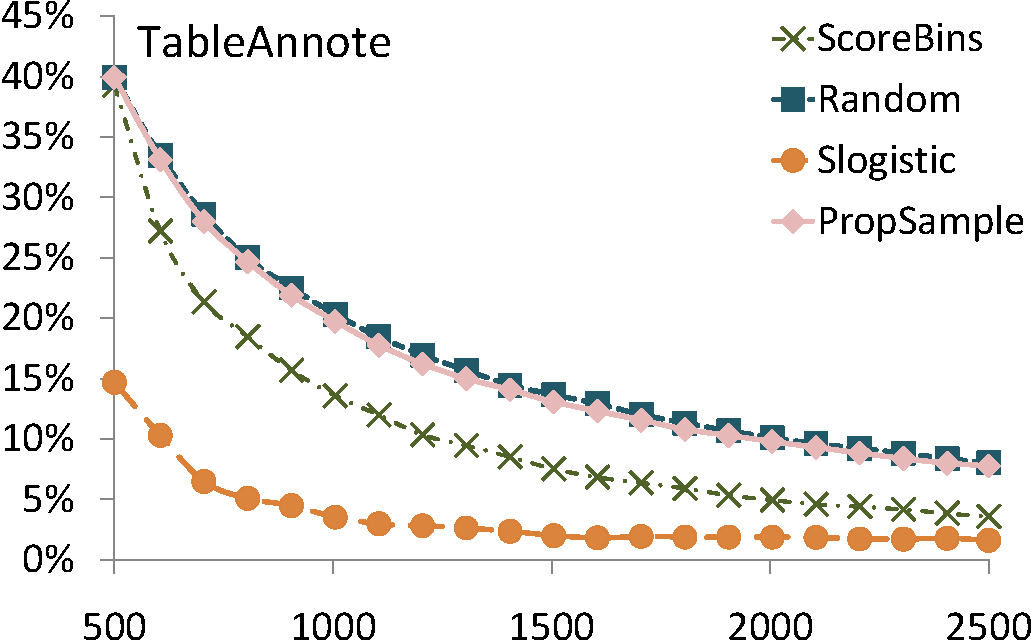
\includegraphics[width=0.5\hsize]{figs/e1tableannote_crop}
\caption{Absolute error (on the $Y$ axis) of different estimation algorithms against no. of labeled instances (on the $X$ axis)}
\end{figure}
\end{center}

\item \textbf{Scalable algorithm} : Perform accuracy estimation on unlabeled data so large that it makes \textcolor{red}{even a single sequential scan impractical} in an interactive setting
\begin{itemize}
\item \textbf{Results} : Able to match within 0.5\% of the estimates of methods based on full scan while sampling just 2.5k instances from indexed unlabeled data
\end{itemize}
\begin{figure}
\begin{center}
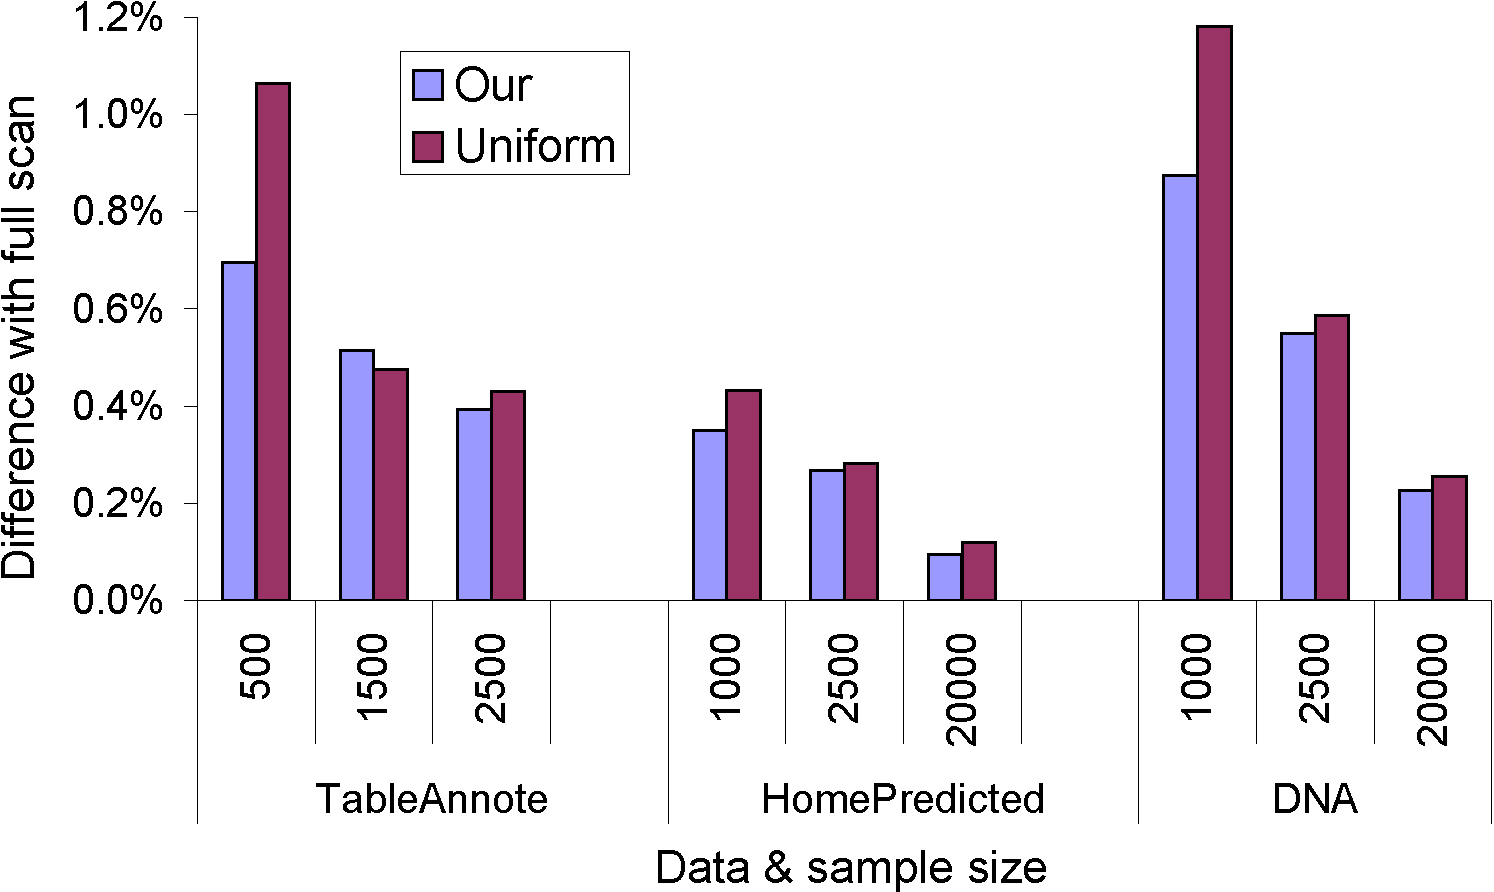
\includegraphics[width=0.46\hsize]{figs/allDataWts-crop}
\caption{Comparing methods of sampling from indexed data for
  estimating bucket weights}
\end{center}
\end{figure}
\end{itemize}
\end{frame}

\section{Background}
\begin{frame}
\frametitle{Motivation}
\begin{itemize}
\item Many applications rely on output of imperfect classifiers deployed on large datasets \\ 
\begin{itemize}
\item \textbf{Examples}: Web page classification, classifying columns of a table to their semantic types
\end{itemize}
\item \textbf{Common characteristics} 
\begin{itemize}
\item Large and diverse dataset 
\item Labeled data unrepresentative of the entire dataset. 
\end{itemize}
\item So \textcolor{red}{Measured accuracy on labeled set $\neq$ True accuracy on data}
\item Hence need a method that can converge to the true accuracy
\begin{enumerate}
\item An algorithm that returns estimate $\estPerf$ of true accuracy $\TP$ of the classifier
\item \textit{Scalable algorithm} : should work on large datasets where sequential scan not possible \& data accessible only via an index
\end{enumerate} 
\end{itemize}
\end{frame}

\begin{frame}
\frametitle{Related Work}
\begin{itemize}
\item Most existing work on \textit{learning} rather than \textit{evaluating} classifiers
\item Existing works on selecting instances for evaluating classifiers:
\begin{itemize}
\item \citep{sawade10} present a new proposal distribution for sampling instances
\item \citep{bennett10} and \citep{druck11} use stratified sampling. However, both assume that classifier $C(\vx)$ is probabilistic \& base their selection on $\Pr(y|\vx)$ scores
\end{itemize}
\item Unlike \citep{bennett10} and \citep{druck11}, \textcolor{red}{instead of fixing a stratification, we learn a new one every time more data gets labeled}
\item None of the existing methods consider cases where the dataset $D$ is too large to even afford a single sequential scan %Our method is designed to perform accuracy estimation and instance selection on D which can only be accessed via an index.
\end{itemize}
\end{frame}

%%%%%%%%%%%%%%%%%%%%%%%%%%%%%%%%%%%%%%%%%%%%%%%%%%%%%%%%%%%%%%%%%%%%%%

\section{Proposed Solution}
\begin{frame}
\frametitle{Overall Idea}
\begin{algorithm}[H]
\begin{spacing}{0.8}
\begin{algorithmic}[1]\itemsep-5pt
\STATE $B=\text{\#buckets},~\vft=\text{feature vector},~\vwa=\text{hyperplanes}$
\STATE $\estSb_b, \wt_b=\text{accuracy \& weight esimates for bucket b}$
\REPEAT
\STATE Learn stratification function $h(\vft|\vwa)$ 
\STATE Stratify $L$ via $h(.)$ \& compute $\{\estSb_b:1\le b \le B\}$
\STATE Stratify $D$ via $h(.)$ \& compute $\{\wt_b:1\le b \le B\}$
\STATE Display accuracy estimates:  $\estSS=\sum\nolimits_b\wt_b\estSb_b$
\STATE Get stratified sample set $L'$ from $D$
\STATE For each $\vx_i \in L'$, get label $y_i$, and add $(\vx_i,y_i)$ to $L$
\UNTIL{accuracy $\estSS$ not converged and labeler not bored.}
\STATE{\bf Return} $\estSS$
\end{algorithmic}
\end{spacing}
\caption{Loop for active accuracy estimation}
\end{algorithm}
\end{frame}

\begin{frame}
\frametitle{Learning a stratification strategy} \vspace{-8mm}
\begin{itemize}
\item Stratify input space so that instances in each stratum have similar accuracy values
\begin{itemize}
\item \emph{Supervised clustering methods} : Learn a distance function \\ \textbf{Issue} : These methods do not scale well 
\item \textbf{Proposal} : Use \textcolor{red}{Hash codes} based on projections on hyperplanes learned over the feature space
\end{itemize}
\item 
\item $\estSb_b=\frac{1}{n_b}\sum_{i\in L_b}\acc_i~$ prone to over-fitting. \textcolor{red}{Smooth based on labeled data in neighbouring buckets}
\item Method agnostic to the type of classifier under consideration
\end{itemize}
\end{frame}

\begin{frame}
\frametitle{Scaling up -- Instance selection on large amounts of data} 
\begin{itemize}
\item TODO: explain where instance selection is needed
\item TODO: describe in a line the idea behind the algorithm to perform accuracy estimation \& instance selection on unlabeled data $D$ which can only be accessed via an efficient index partition 
\end{itemize}
\end{frame}

%%%%%%%%%%%%%%%%%%%%%%%%%%%%%%%%%%%%%%%%%%%%%%%%%%%%%%%%%%%%%%%%%%%%%%
\section{Results}
\begin{frame}[allowframebreaks]{Results}
\begin{center}
\begin{table}
\centering
\begin{small}
\begin{tabular}{|l@{}|@{}r|@{}r|@{}r|@{}r|@{}r|}
\hline
Dataset & \multicolumn{1}{c}{\#} \vline & \multicolumn{2}{c}{Size} \vline & \multicolumn{2}{c}{Accuracy (\%)} \vline \\
 & \multicolumn{1}{c}{Features} \vline & \multicolumn{1}{c}{Seed($L$)} \vline & \multicolumn{1}{c}{Unlabeled($D$)} \vline & \multicolumn{1}{r}{Seed($L$)} \vline & \multicolumn{1}{r}{True($D$)} \vline \\
\hline
TableAnnote & 42 & 541 & 11,954,983 & 56.4 & 16.5 \\
Spam & 1000 & 5000 & 350,000 & 86.4 & 93.2 \\
DNA & 800 & 100,000 & 50,000,000 & 72.2 & 77.9 \\
HomeGround & 66 & 514 & 1060 & 50.4 & 32.8 \\
HomePredicted & 66 & 8658 & 13,951,053 & 83.2 & 93.9 \\
\hline
\end{tabular}
\end{small}
\caption{Summary of Datasets}
\end{table}
\end{center}

\framebreak

\begin{center}
\begin{figure}
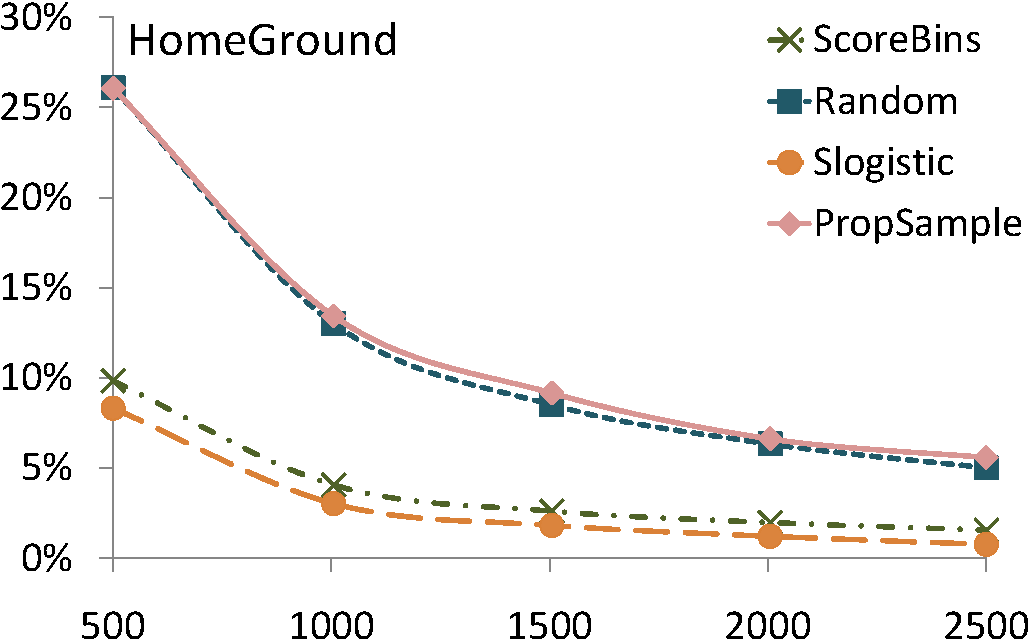
\includegraphics[width=0.82\hsize]{figs/e1homeground_crop}
\caption{Homeground data: Absolute error ($Y$ axis) of different estimation algorithms against increasing number of labeled instances ($X$ axis)}
\end{figure}

\framebreak

\begin{figure}
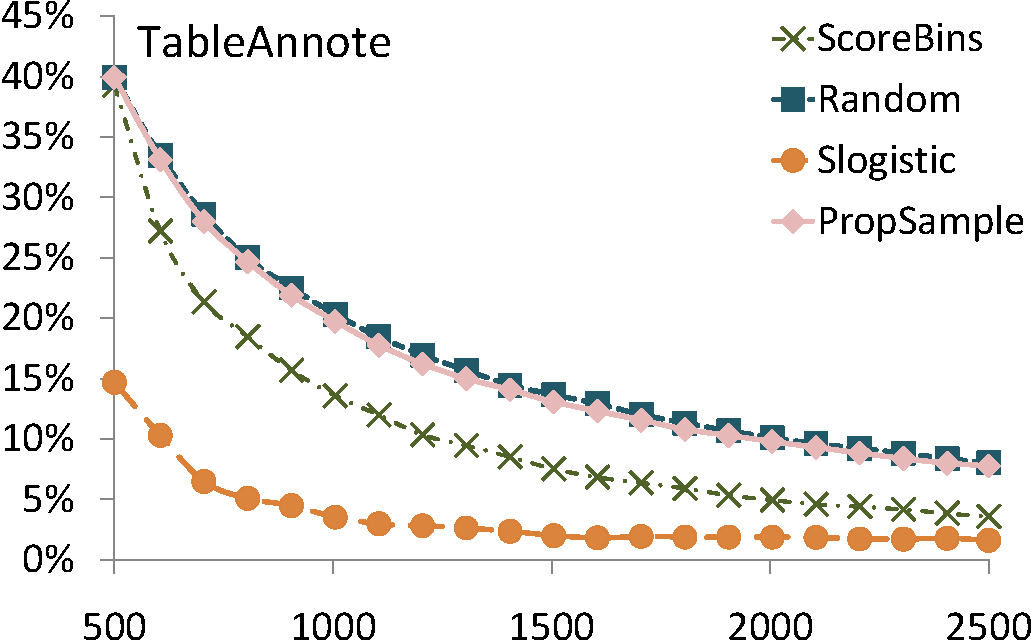
\includegraphics[width=0.37\hsize]{figs/e1tableannote_crop}
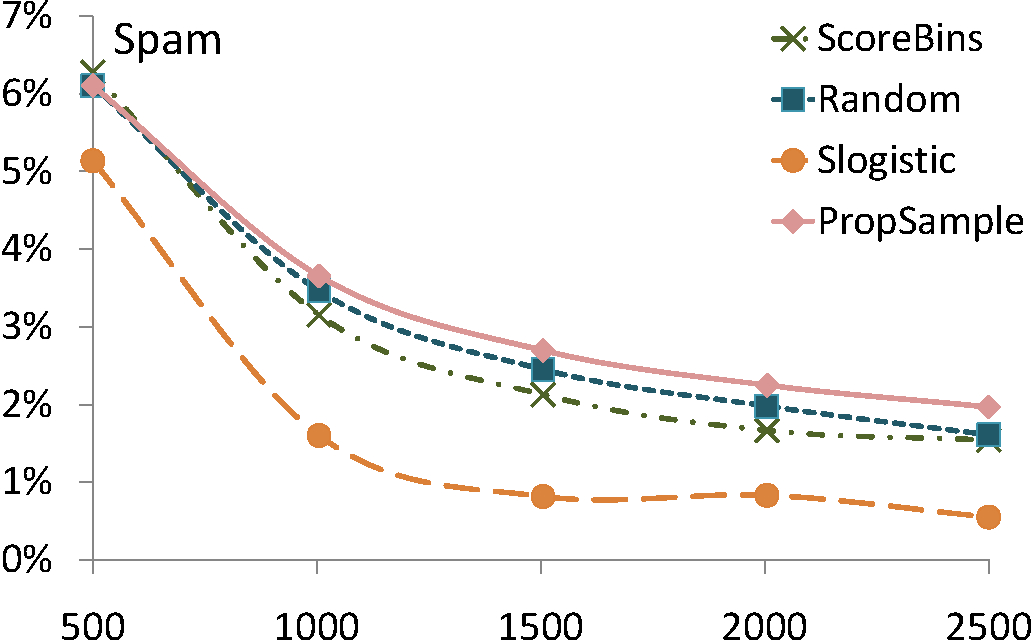
\includegraphics[width=0.37\hsize]{figs/e1spam_crop}
\end{figure}
\begin{figure}
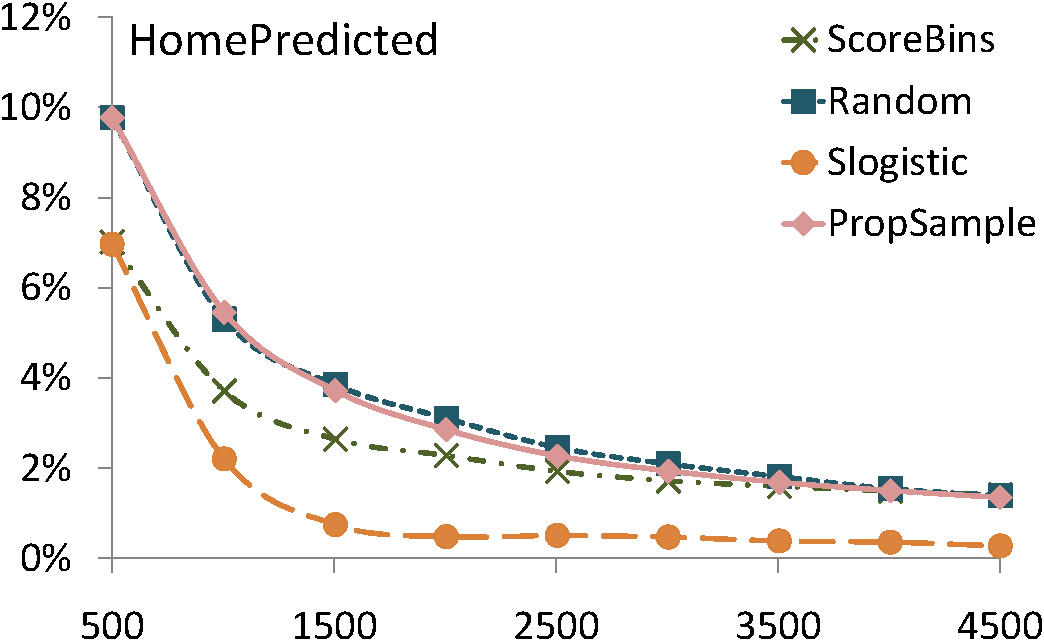
\includegraphics[width=0.37\hsize]{figs/e1homepredicted_crop}
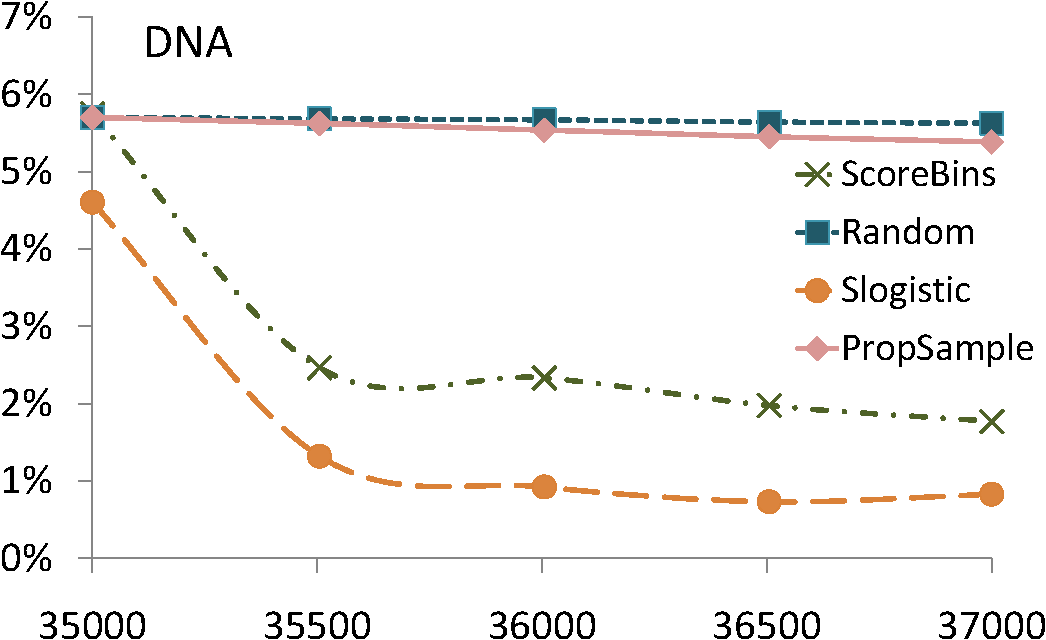
\includegraphics[width=0.37\hsize]{figs/e1dna_crop}
\caption{Absolute error (on the $Y$ axis) of different estimation algorithms against increasing number of labeled instances (on the $X$ axis)}
\end{figure}
\end{center}

\framebreak

\begin{center}
\begin{figure}
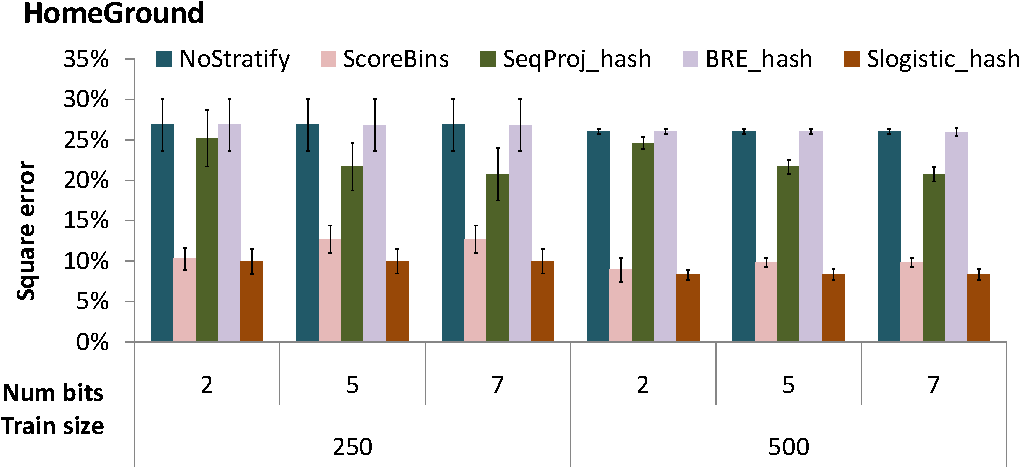
\includegraphics[width=\hsize]{figs/e2homeground_crop}
\caption{HomeGround data: Error of different stratification methods against increasing
  training sizes \& for different number of bits}
\end{figure}

\framebreak

\begin{figure}
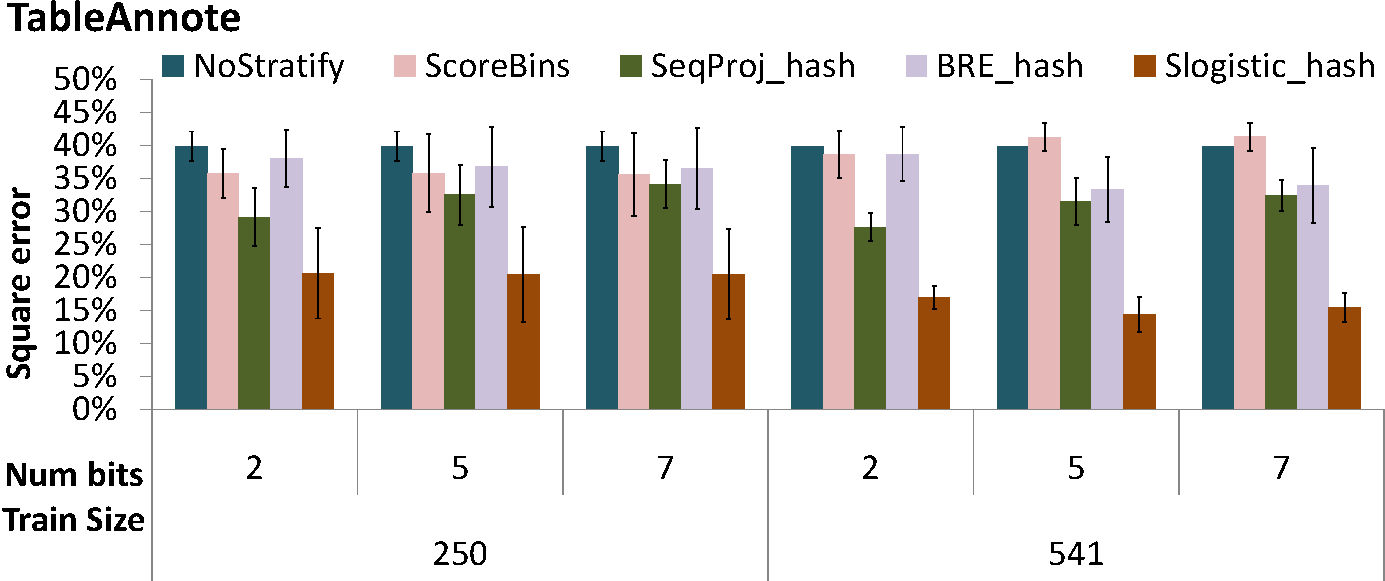
\includegraphics[width=0.5\hsize]{figs/e2tableannote_crop}
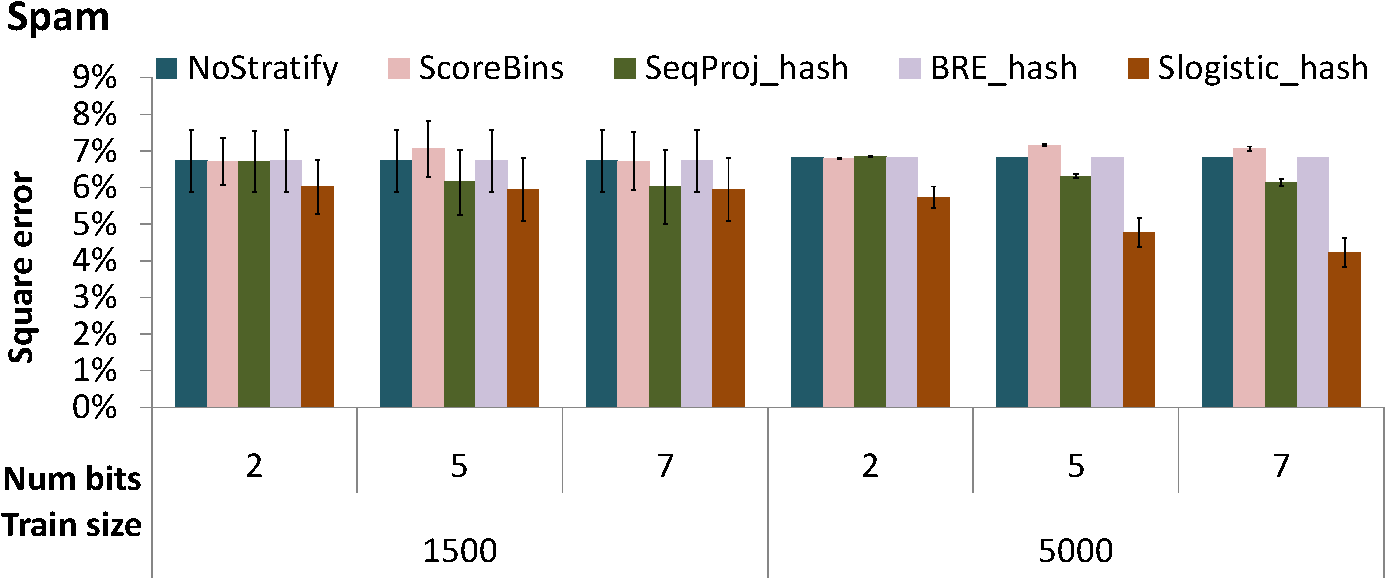
\includegraphics[width=0.5\hsize]{figs/e2spam_crop}
\end{figure}
\begin{figure}
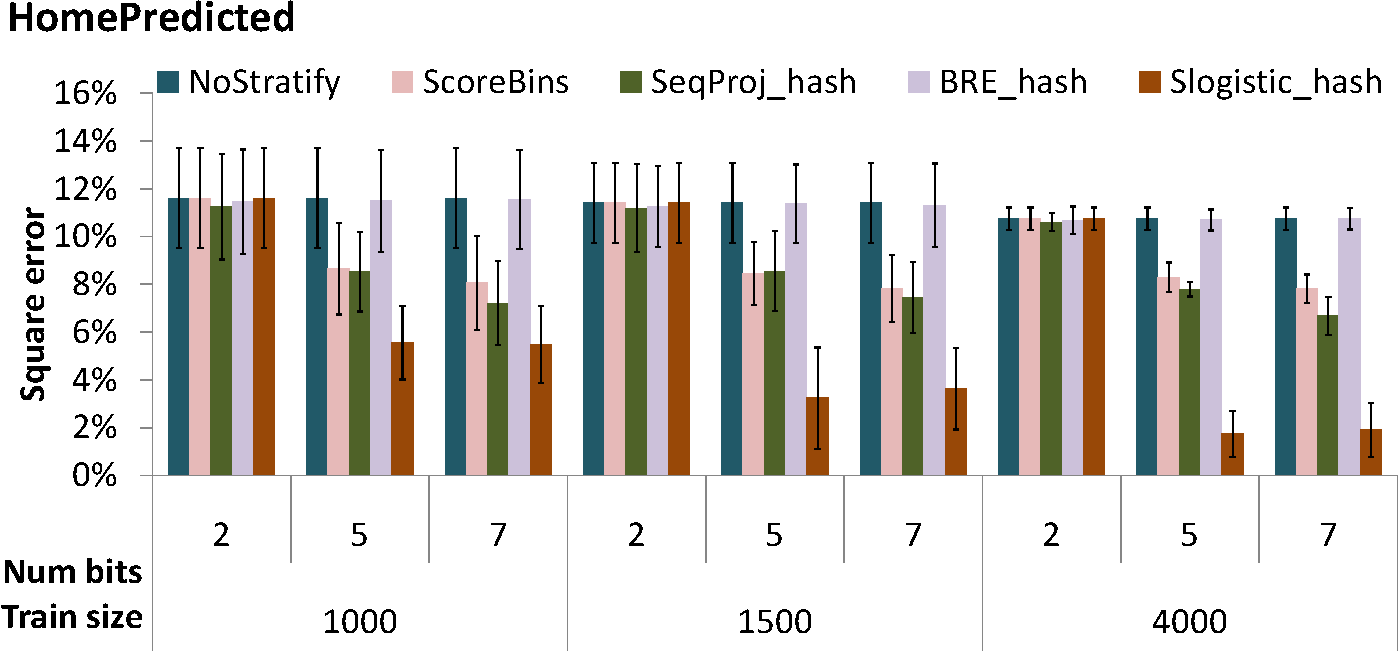
\includegraphics[width=0.5\hsize]{figs/e2homepredicted_crop}
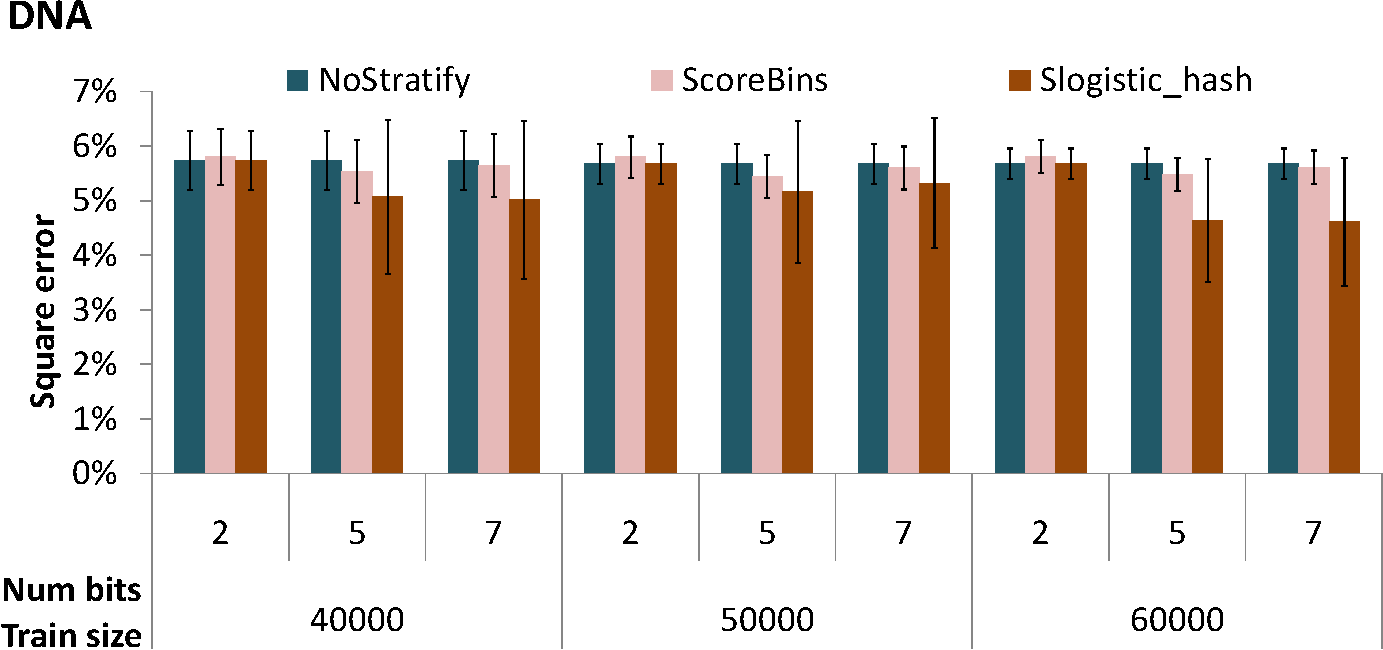
\includegraphics[width=0.5\hsize]{figs/e2dna_crop}
\caption{Error of different stratification methods against increasing
  training sizes and for different number of bits}
\end{figure}
\end{center}

\framebreak

\begin{figure}
\begin{center}
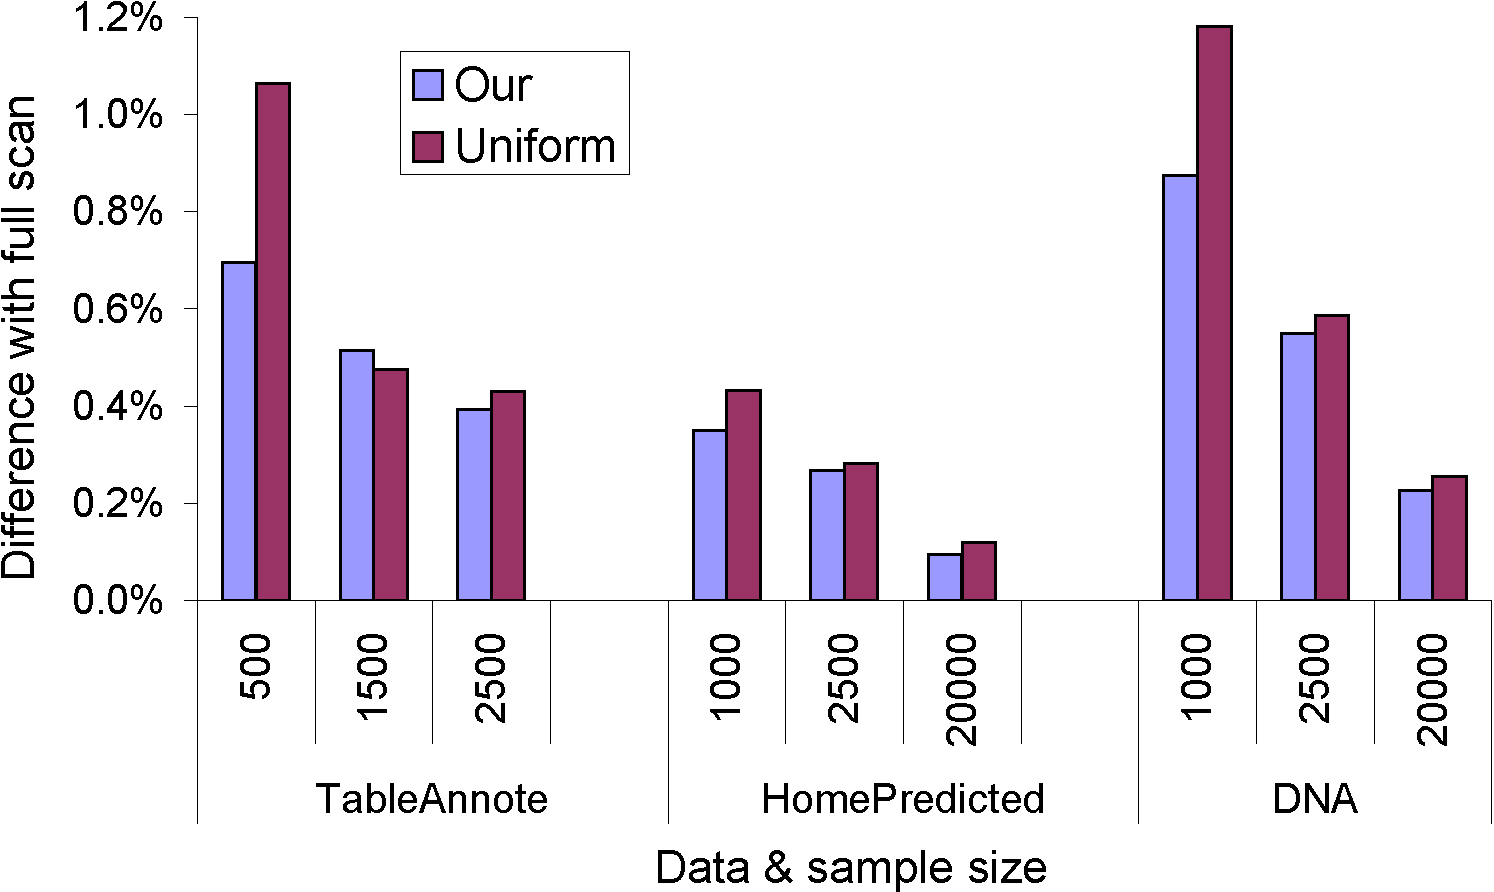
\includegraphics[width=0.85\hsize]{figs/allDataWts-crop}
\caption{Comparing methods of sampling from indexed data for
  estimating bucket weights}
\label{fig:allWts}
\end{center}
\end{figure}

\end{frame}

%%%%%%%%%%%%%%%%%%%%%%%%%%%%%%%%%%%%%%%%%%%%%%%%%%%%%%%%%%%%%%%%%%%%%%

\section{Summary \& Conclusions}
\begin{frame}{Summary}
\begin{enumerate}
\item Addressed the challenge of \emph{calibrating a classifier's accuracy on large unlabeled datasets given small amounts of labeled data and a human labeler}
\item Proposed a stratified sampling-based method that provides better estimates than simple averaging \& better selection of instances for labeling than random sampling 
\item Between 15\% and 62\% relative reduction achieved in error compared to existing approaches
\item Algorithm made \emph{scalable} by proposing optimal sampling strategies for accessing indexed unlabeled data directly
\item Close to optimal performance while reading three orders of magnitude fewer instances on large datasets 
\end{enumerate}
\end{frame}

\begin{frame}
\frametitle{}
\begin{center}
\LARGE{Thank You}
\end{center}
\end{frame}

%%%%%%%%%%%%%%%%%%%%%%%%%%%%%%%%%%%%%%%%%%%%%%%%%%%%%%%%%%%%%%%%%%%%%%

% \section{References}
\begin{frame}[allowframebreaks]{References}
\bibliography{report}
\end{frame}
\end{document}

%% \subsection{Related Work}
%\begin{frame}
%\frametitle{Related Work}
%\begin{itemize}
%\item \textit{Online Stratified Sampling: Evaluating Classifiers at Web-Scale \cite{bennett10}}
%\begin{itemize}
%\item Disproportionate optimal sampling ($n_b \propto \hat{\sigma_b}$) 
%\item Assume classifier score
%\item Divide the score range into equal sizes -- stratifying into contiguous classifier score intervals breaks distribution into segments that
%are more homogeneous on average than the overall distribution
%\end{itemize}
%\item \textit{Toward Interactive Training and Evaluation \cite{druck11}} 
%\begin{itemize}
%\item Very similar to \cite{bennett10} -- however the estimation method is generalized to structured output spaces as well
%\end{itemize}
%\item \textit{Active Risk Estimation \cite{sawade10}}
%\begin{itemize}
%\item Sample using a proposal distribution: $\estProp = \frac{1}{\sum_i \frac{1}{q(\vx_i)}} \sum\nolimits_i \frac{\acc_i}{q(\vx_i)}$
%\item However optimal $q(\vx)$ depends on the unknown true accuracy $\TP$ and the unknown true distribution $\Pr(y|\vx)$.
%\item $\TP~\leftarrow$ Introspective accuracy 
%\item $\Pr(y|\vx)~\leftarrow~C(\vx)$ assumed to be a probabilistic classifier that provides an estimate of the true $\Pr(y|\vx)$.  
%\end{itemize}
%\end{itemize}
%\end{frame}
%
%%%%%%%%%%%%%%%%%%%%%%%%%%%%%%%%%%%%%%%%%%%%%%%%%%%%%%%%%%%%%%%%%%%%%%%%%%%%%%%%
%
%\section{Active Accuracy Estimation}
%% \subsection{Algorithm}
%\begin{frame}
%\frametitle{Algorithm Overview}
%\begin{center}
%\textsc{Loop for active accuracy estimation}
%\end{center}
%\begin{algorithmic}[1]
%\STATE {\bf Input} $L,D,k,R,B$
%\REPEAT
%\STATE Learn stratification function $h(\vx|\vw) \mapsto [1\ldots B]$ if more than $R$ instances labeled since last training
%\STATE Compute $\{\estSb_b:1\le b \le B\}$ from $L$ 
%\STATE Compute $\{\wt_b:1\le b \le B\}$ from $D$
%\STATE Display estimates:  $\estSS=\sum\nolimits_b\wt_b\estSb_b$.
%\STATE Select set $S$ of $k$  instances from $D$ (Using the static index)
%\STATE For each $\vx_i \in S$, get label $y_i$, and add $(\vx_i,y_i)$ to $L$.  
%% compute $a_i=\acc(y_i,C(\vx_i))$ 
%\UNTIL{accuracy not converged and labeler not bored.}
%\end{algorithmic}
%\end{frame}
%
%% \subsection{Subproblems}
%\begin{frame}[allowframebreaks]
%\frametitle{Subproblems}
%\begin{enumerate}
%\item \textbf{Learning Stratification Function}
%\begin{itemize}
%\item Learn $\nb = \log B$ hash functions $h_1,\ldots,h_\nb$ 
%such that each $h_j(\vx)$ maps an instance to 0 or 1, and the concatenation of
%the $\nb$ bits gives the stratum number of an instance.
%\item  Reduces to learning $\nb$ hyperplanes $\vw_1,\ldots,\vw_\nb$ --
%instances lying on same side of all hyperplanes have 
%similar accuracy values.
%\end{itemize}
%
%\item \textbf{Estimating Accuracy of a Stratum}
%\begin{itemize}
%\item Depend on just the labeled instances in a stratum might lead to over-fitting in strata with very few labeled examples
%\item Smooth estimates based on labeled data in neighboring buckets : $\estSb_b=\frac{n^+_b + \gamma\sum_{d=1}^\nb\beta^d\sum_{b':\ham(b,b')=d}n^+_{b'}}
%{n_b + \gamma\sum_{d=1}^\nb\beta^d\sum_{b':\ham(b,b')=d}n_{b'}}$ \\
%We used $\gamma=5$, and $\beta=0.1$ for our experiments
%\end{itemize}
%
%\framebreak
%
%\item \textbf{Estimating weight of each stratum}
%\begin{itemize}
%\item We need to find fraction $\wt_b$ of instances from $D$ that
%lie in each stratum $b$.  
%\item When size of $D$ is small, a single pass over the data yields $\wt_b=\frac{1}{N}\sum\nolimits_{\vx \in D}\indicate{h(\vx|\vw)=b}$ for each $b$.
%How these weights are computed using the index on the data, without accessing the entire data every time $h(\vx|\vw)$ is retrained, is discussed later
%\end{itemize}
%
%\item \textbf{Selecting instances for labeling}
%\begin{itemize}
%\item The optimal method is to perform importance sampling on
%$D$ where importance of an instance $\vx$ is proportional to $\estVar_{h(\vx)}$. 
%\item If $D$ is explicitly partitioned as per $h(\vx)$ : Selecting a bucket with probability
%proportional to $\wt_b\estVar_b$ and then select an instance within $b$ with equal probability. 
%\item For large $D$, this sampling, without stratifying the entire $D$, is performed using the static index on the data.
%\end{itemize}
%\end{enumerate}
%\end{frame}
%
%%%%%%%%%%%%%%%%%%%%%%%%%%%%%%%%%%%%%%%%%%%%%%%%%%%%%%%%%%%%%%%%%%%%%%%
%
%\section{Learning Hyperplanes}
%% \subsection{Goals}
%\begin{frame}
%\frametitle{Learning Hyperplanes}
%\begin{itemize}
%\item Learn hyperplanes $\vw_1,\ldots,\vw_\nb$ which will be used to hash partition the data
%\item Minimize the expected square error of estimate $\estSS$ which is $\sum\nolimits_b\wt_b^2\tfrac{\estVar_b^2}{n_b}$
%\item \textit{Related recent work} : Learning hash functions where objective stated in terms of distances between pairs of instances. \\ 
%\textit{Popular variant} : Distance scores between instance pairs provided. Hash functions learnt such that Hamming distance over learned signatures correlates with given distance scores
%\item \textbf{Result} : If $p_b \propto n_b$, then $\sum_b\wt_b^2\tfrac{\estVar_b^2}{n_b}=\sum_b\tfrac{1}{n^2n_b}\sum_{\vx_i,\vx_j \in L_b}(\acc_i-\acc_j)^2$.
%\end{itemize}
%\end{frame}
%
%% \subsection{Review of Hash Learning Techniques}
%\begin{frame}
%\frametitle{Hash Learning Techniques}
%\begin{itemize}
%\item Min-Loss Hashing \cite{norouzi2011minimal} 
%\begin{itemize}
%\item Hinge-like loss function
%\item Objective smoothed by piecewise linear upper bound as in \cite{tsochantaridis05}
%\item For us, local minimas were very bad \& we could not progress beyond the initial step with both random and all-zero initialization of $\vw$ values
%\end{itemize}
%
%\item Binary Reconstructive Embedding \cite{kulis2009learning}
%\begin{itemize}
%\item Updates a single hyperplane parameter at a time optimally in a coordinate ascent loop
%\item We found the single parameter update strategy to be very slow for our task
%\end{itemize}
%
%\item Sequential Projection Learning \cite{wang2010sequential}
%\begin{itemize}
%\item Sequentially learns each hyperplane optimally in a block coordinate ascent loop
%\item Replace sign($\cdot$)  with signed magnitude in the objective
%\item First eigenvector of transformed data matrix
%\item Reweight instances misclassified by previously learnt hyperplanes
%\end{itemize}
%
%\end{itemize}
%\end{frame}
%
%% \subsection{Signed Logistic Hashing}
%\begin{frame}[allowframebreaks]
%\frametitle{Signed Logistic Hashing}
%\begin{itemize}
%\item Initialize hyperplanes \& update single hyperplane at a time on re-weighted set of instances until local minima is reached
%\item Fix $r-1$ hyperplanes -- training data partitioned into $B/2$ groups $L_1,\ldots,L_{B/2}$. Using remaining hyperplane, bisect each partition $L_k$ into 2 parts $L^1_k$ and $L^2_k$ so that sum of error over the new $B$ buckets minimized
%\item Error of bucket $b$ =  $n_b\estVar_b^2$ 
%\item For binary $a$, $\estVar_b^2 = \posf_b(1-\posf_b)$ where $\posf_b$ = fraction of labeled instances $i$ in bucket $b$ with $\acc_i=1$
%\item Let $\Err(\vw,L_k)$ denote sum of error of buckets $L^1_k$ and $L^2_k$ created on bisecting group $L_k$ using
%$\vw$. Clearly, $\Err(\vw,L_k) = \np\fp(1-\fp) + \nn\fn(1-\fn)$ Non-differentiable \& non-convex objective
%\framebreak
%\item Let $\loss(a_i,\vw\cdot\vx_i)$ = convex upper bound to $\sign(\vw\cdot\vx_i)$ Then,  $\Err(\vw,L_k) \le \min(\sum_{\vx^i \in L_k}\loss(1-a_i,\vw\cdot\vx_i), \sum_{\vx^i \in L_k}\loss(a_i,\vw\cdot\vx_i))$
%\item \textit{Relaxed Objective} : $\min_{\vw}\sum_{k=1}^{B/2}\min(\sum_{\vx^i \in L_k}\loss(1-a_i,\vw\cdot\vx_i), \sum_{\vx^i \in L_k}\loss(a_i,\vw\cdot\vx_i))$
%\item Solve using a EM-like algorithm
%\begin{itemize}
%\item Assume for each group $k$, we know $z_k$ a function on $a$ returns either identity $a$ or negation $1-a$ 
%\item Consider objective $\min_{\vw}\sum\nolimits_{k=1}^{B/2}\sum\nolimits_{\vx^i \in L_k}\loss(z_k(a_i),\vw\cdot\vx_i)$
%\item Start with some initial guess of $z_k$ = identity and find a $\vw$
%\item For a fixed $\vw$, find optimal $z_k$ that minimizes loss of group $k$
%\item Continue until convergence to a local minima
%\end{itemize}
%\framebreak
%\item \textbf{Initializing hyperplanes} : Hierarchical partitioning of data
%\begin{itemize}
%\item Initially, entire data in a single group 
%\item Find hyperplane that partitions the group so as to minimize $\loss()$ on the group 
%\item Repeat following in a loop $B-1$ times : Find largest $m$ groups and for each group $g$ invoke the binary classifier to minimize $\loss()$ on $g$.  Pick best of these $m$ hyperplanes (best = minimize sum of error over all current buckets)
%\end{itemize}
%\item \textbf{Reweighting instances}
%\begin{itemize}
%\item $\minor(L_k)$ = minority class in $L_k$, \\ $e_k$ = fraction of instances $\vx_i \in L_k$ for which $\acc_i=\minor(L_k)$
%\item Interpret $e_k$ as error incurred on $L_k$ from previous hyperplanes 
%\item Assign weights $u_i$ to each instance $\vx_i \in L_{k}$ as $u_i=\frac{1-e_k}{e_k}~ \text{if} ~a_i = \minor(L_k)$ else $u_i=1$
%\end{itemize}
%\framebreak
%\begin{center}
%\textsc{Signed Logistic Hashing}
%\end{center}
%\begin{algorithmic}
%\STATE $\vw^0_1 \cdots \vw^0_r$ = Initial hyperplanes
%\WHILE{estimated error reduces}
%\FOR{$j=1$ to $r$}
%\STATE $u_i$ = weight of instance $i$  as discussed
%\STATE $z_k=$Id for all $B/2$ groups of $L$ after $\vw_j$ is removed.
%\WHILE{$z_k$ changes} 
%\STATE  $\vw_j = \argmin_{\vw}\sum\nolimits_{k=1}^{B/2}\sum\nolimits_{\vx^i \in L_k}u_i\loss(z_k(a_i),\vw\vx_i)$
%\STATE $z_k = \argmin_{z = \text{Id,Neg}}\sum\nolimits_{\vx^i \in L_k}\loss(z(a_i),\vw\vx_i)$
%\ENDWHILE
%\ENDFOR
%\ENDWHILE
%\end{algorithmic}
%\end{itemize}
%\end{frame}
%
%%%%%%%%%%%%%%%%%%%%%%%%%%%%%%%%%%%%%%%%%%%%%%%%%%%%%%%%%%%%%%%%%%%%%%%
%
%\section{Sampling on Indexed Data}
%% \subsection{Introduction}
%\begin{frame}
%\frametitle{Sampling on Indexed Data}
%\begin{itemize}
%\item Unlabeled data accessed in 2 different steps of our algorithm
%\begin{itemize}
%\item Calculating fraction $\wt_b$ of instances belonging to each
%bucket $b$; these weights in turn are used to estimate accuracy
%\item When selecting instances for labeling we perform importance sampling where imp($\vx$) $\propto \estVar_{h(\vx)}$. Cannot do a sequential scan over $D$ every time hash function $h(\vx)$ is retrained
%\end{itemize}
%\item \textit{Assumption}: Unlabeled data $D$ indexed so as to partition data into disjoint parts $D_1,\ldots,D_U$. For each
%partition $u$ we can 
%\begin{itemize}
%\item Get its size $N_u$ in terms of number of instances, and 
%\item Generate a uniform random sample of instances within the partition.
%\end{itemize}
%\end{itemize}
%\end{frame}
%
%% \subsection{Assigning bucket weights}
%\begin{frame}
%\frametitle{Assigning Bucket Weights}
%\begin{itemize}
%\item Sample from a proposal distribution : $\hat{A}_{S_q} = \frac{1}{|S|}\sum\nolimits_{\vx\in S} \frac{1/N}{q(\vx)}\estSb_{h(\vx)}$
%\item \textbf{Result} : When $q(\vx)$ is restricted so that all instances within a partition $u$ are sampled with the same probability $q_u$,
%the expected squared error between $\hat{A}_{S_q}$ and $\estSS$ is minimized when 
%\begin{center} $q_u \propto \sqrt{\sum_{b}\estSb^2_b\wt(b|u)}$ \end{center}
%\item $\wt(b|u)$ = fraction of instances in $D_u$ with $h(\vx)=b$
%\item Initially, use labeled data to estimate $\wt(b|u)$
%\item As more instances are sampled from any $D_u$, refine estimates of $\wt(b|u)$
%\end{itemize}
%\end{frame}
%
%% \subsection{Instance Selection}
%\begin{frame}
%\frametitle{Instance Selection}
%\begin{itemize}
%\item Perform importance sampling where imp($\vx$) $\propto \estVar_{h(\vx)}$ without evaluating $h(\vx)$ over entire $D$
%\item Generate a larger sample $S$ via proposal distribution $q(\vx)$ restricted to choose same $q(\vx) ~\forall \vx$ in data
%partition $D_u$ 
%\item Then from $S$ generate the sample of $k$ instances by weighting each instance as $f(\vx)/q(\vx)$. Good only if $q(\vx) \sim f(\vx)$
%\item Best $q(\vx)$ found by solving for unlabeled bucket weights $q_1,\ldots,q_U$
%so that expected L1 distance between $f(\vx)$ and $q(\vx)$ is minimized
%\begin{center}
%$\min_{q_1,\ldots,q_U} \sum_u\sum_b \wt_u\wt(b|u) \left|\frac{\estVar_b}{Z_f} - q_u\right| ~s.t. \sum_u N\wt_uq_u=1$
%\end{center}
%\item $Z_f$ approximated as $\sum\nolimits_b\estVar_b\sum\nolimits_u\wt_u\wt(b|u)$
%\item Get $\wt(b|u)$ as explained in the previous slide
%\end{itemize}
%\end{frame}
%
%%%%%%%%%%%%%%%%%%%%%%%%%%%%%%%%%%%%%%%%%%%%%%%%%%%%%%%%%%%%%%%%%%%%%%%
%
%\section{Experiments}
%% \subsection{Overall Comparison}
%\begin{frame}
%\frametitle{Experiments : Overall Comparison}
%\begin{center}
%\textsc{Error of different estimation algorithms against increasing number of labeled instances} 
%\end{center}
%\begin{center}
%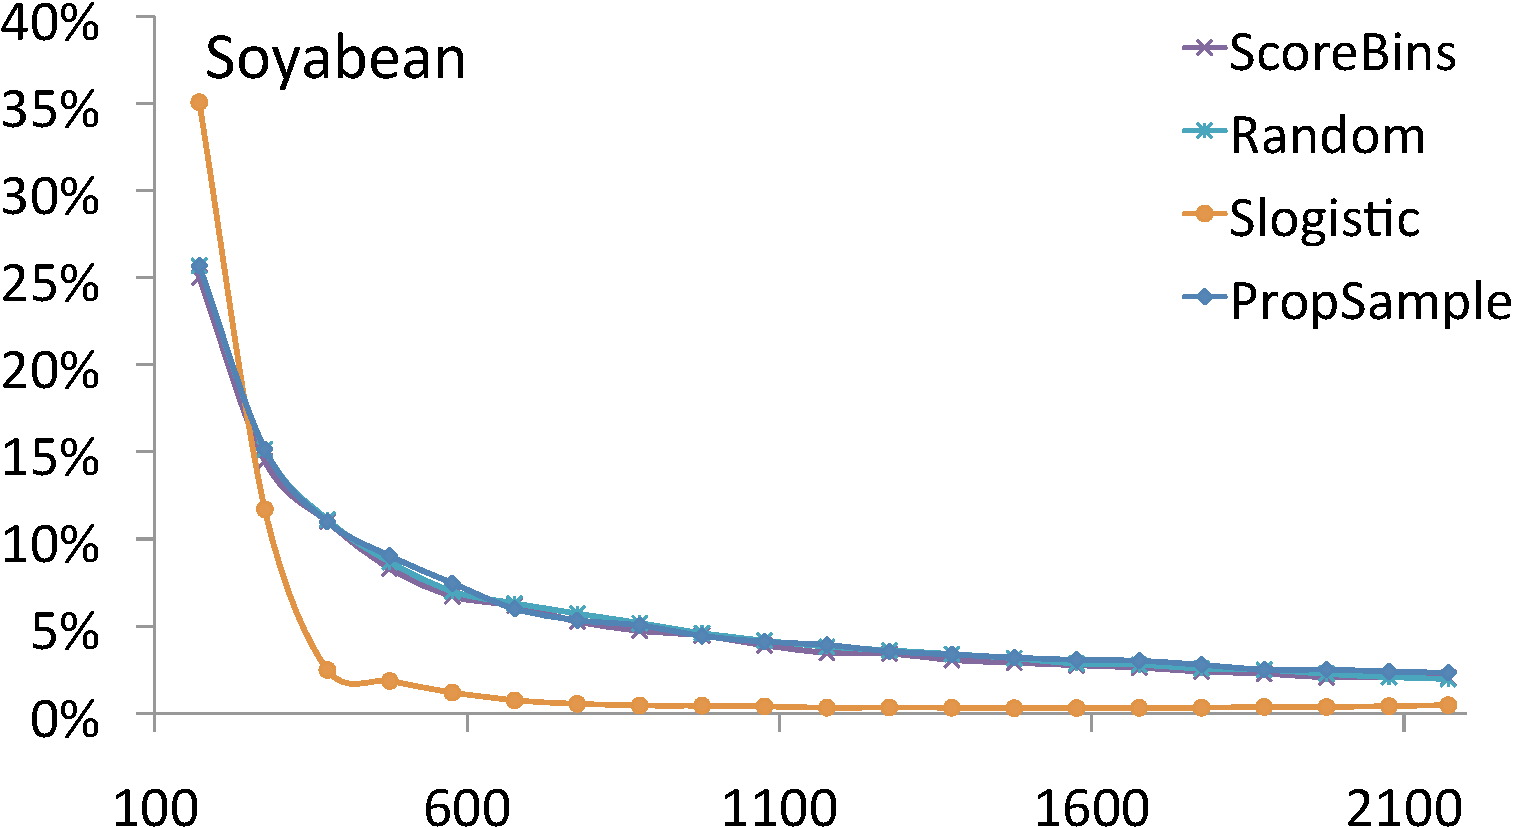
\includegraphics[width=0.34\hsize]{figs/e1wekacrop}
%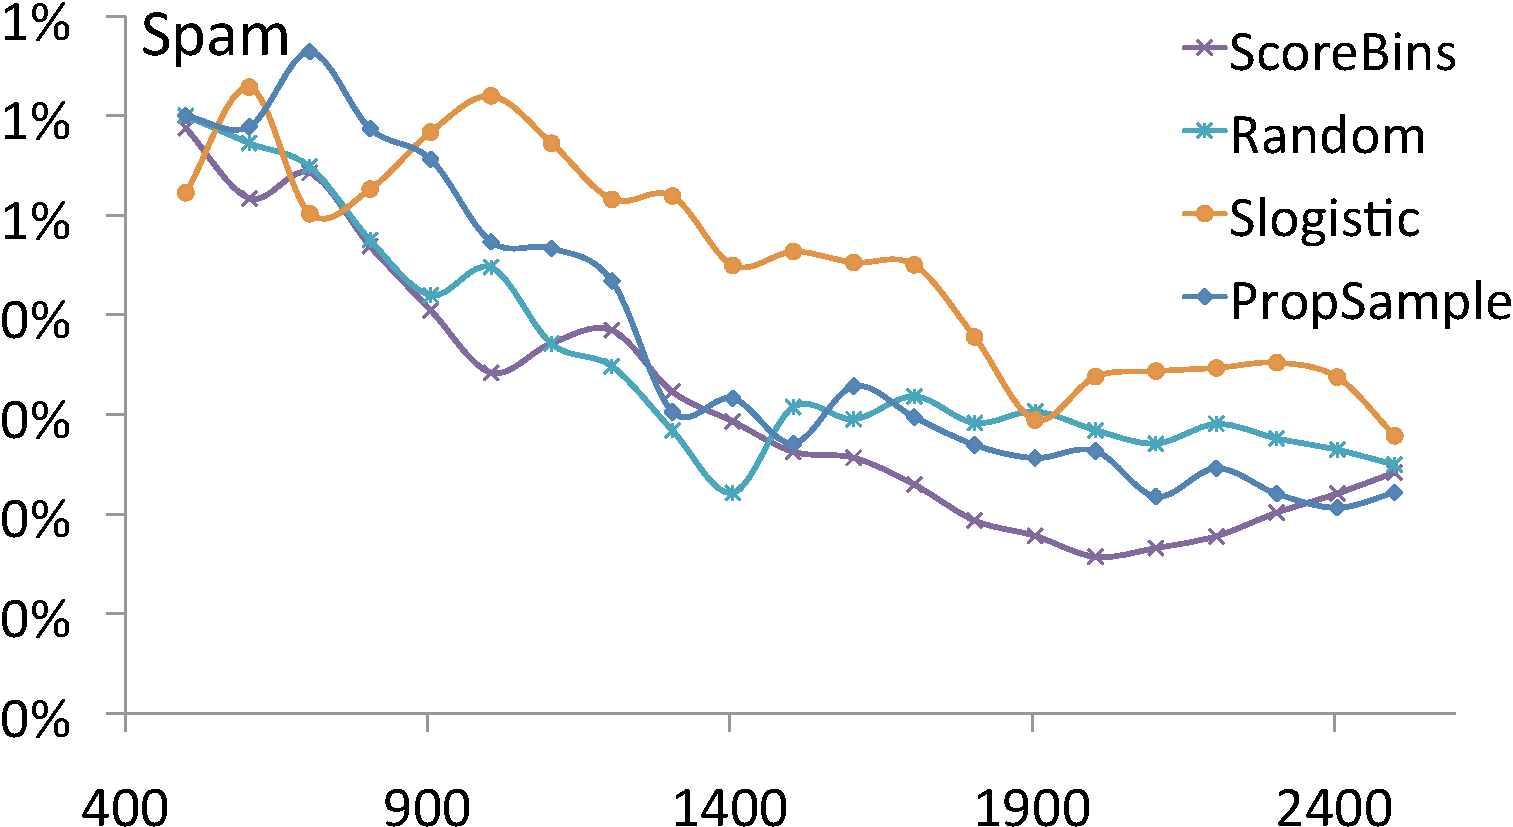
\includegraphics[width=0.34\hsize]{figs/e1webspamcrop}
%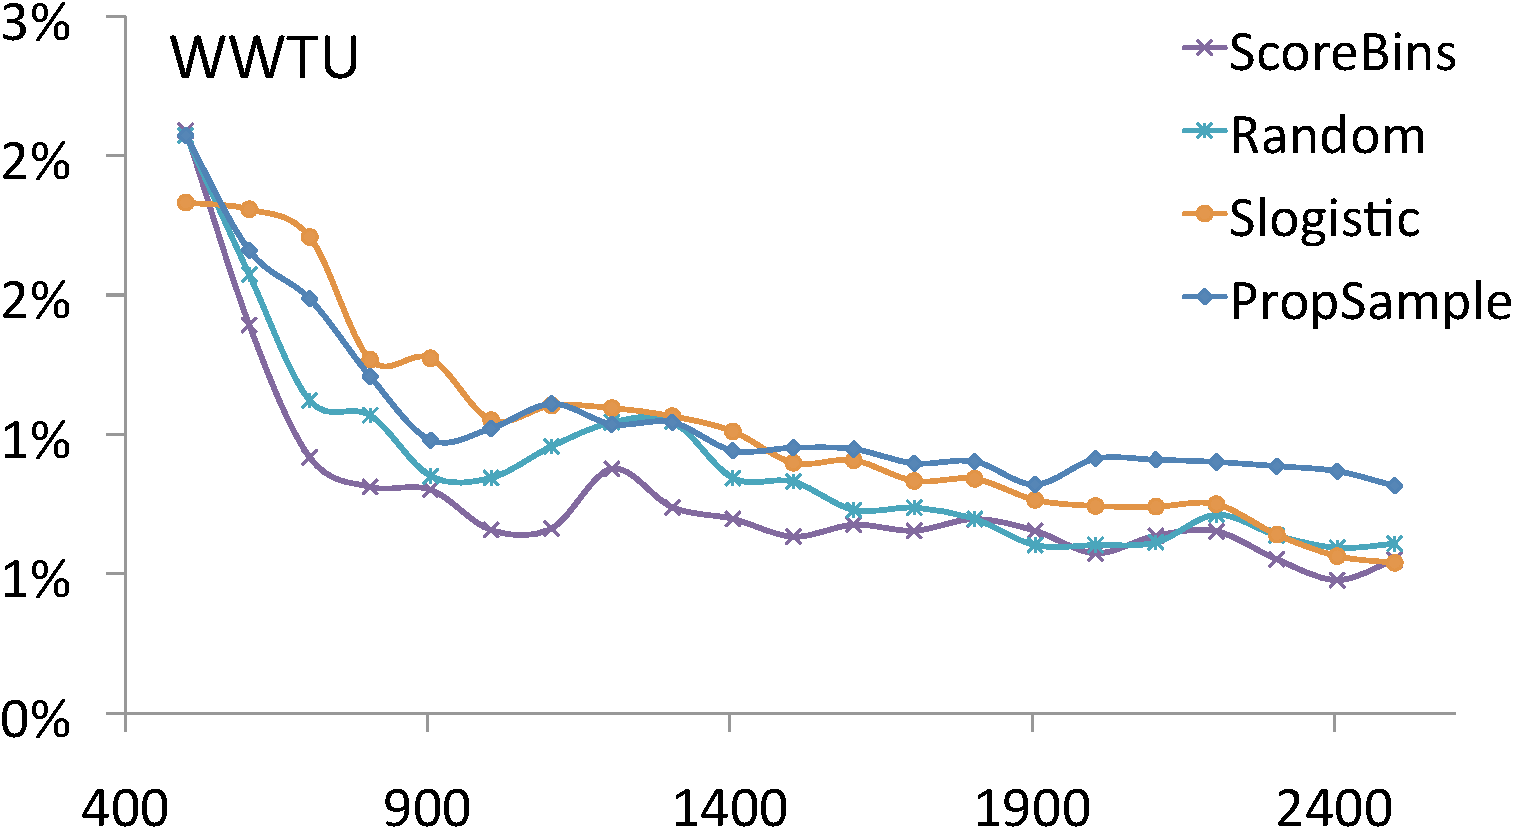
\includegraphics[width=0.34\hsize]{figs/e1wwtucrop}
%\end{center}
%\begin{center}
%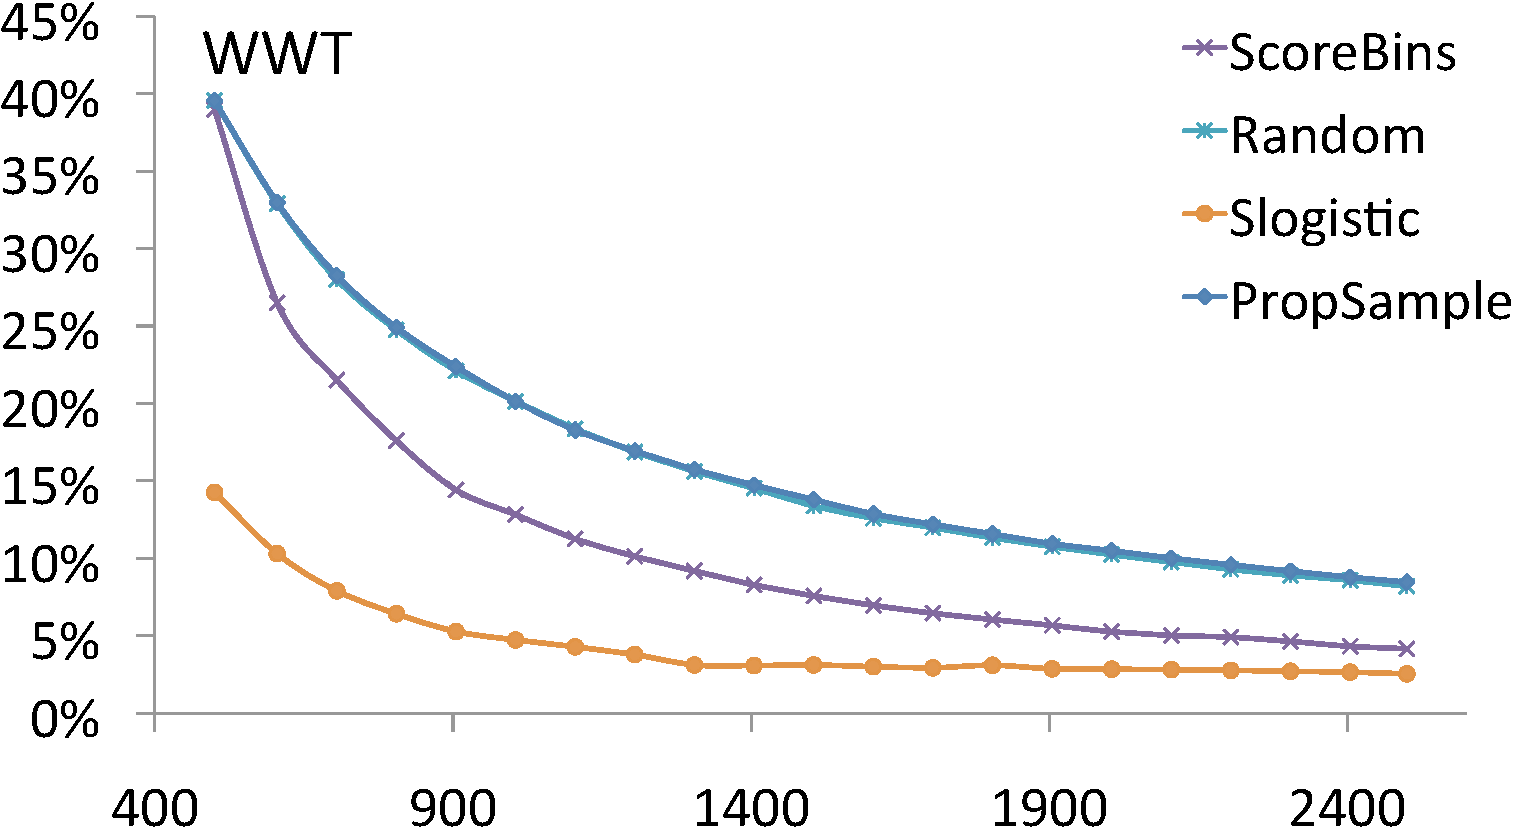
\includegraphics[width=0.35\hsize]{figs/e1wwtcrop}
%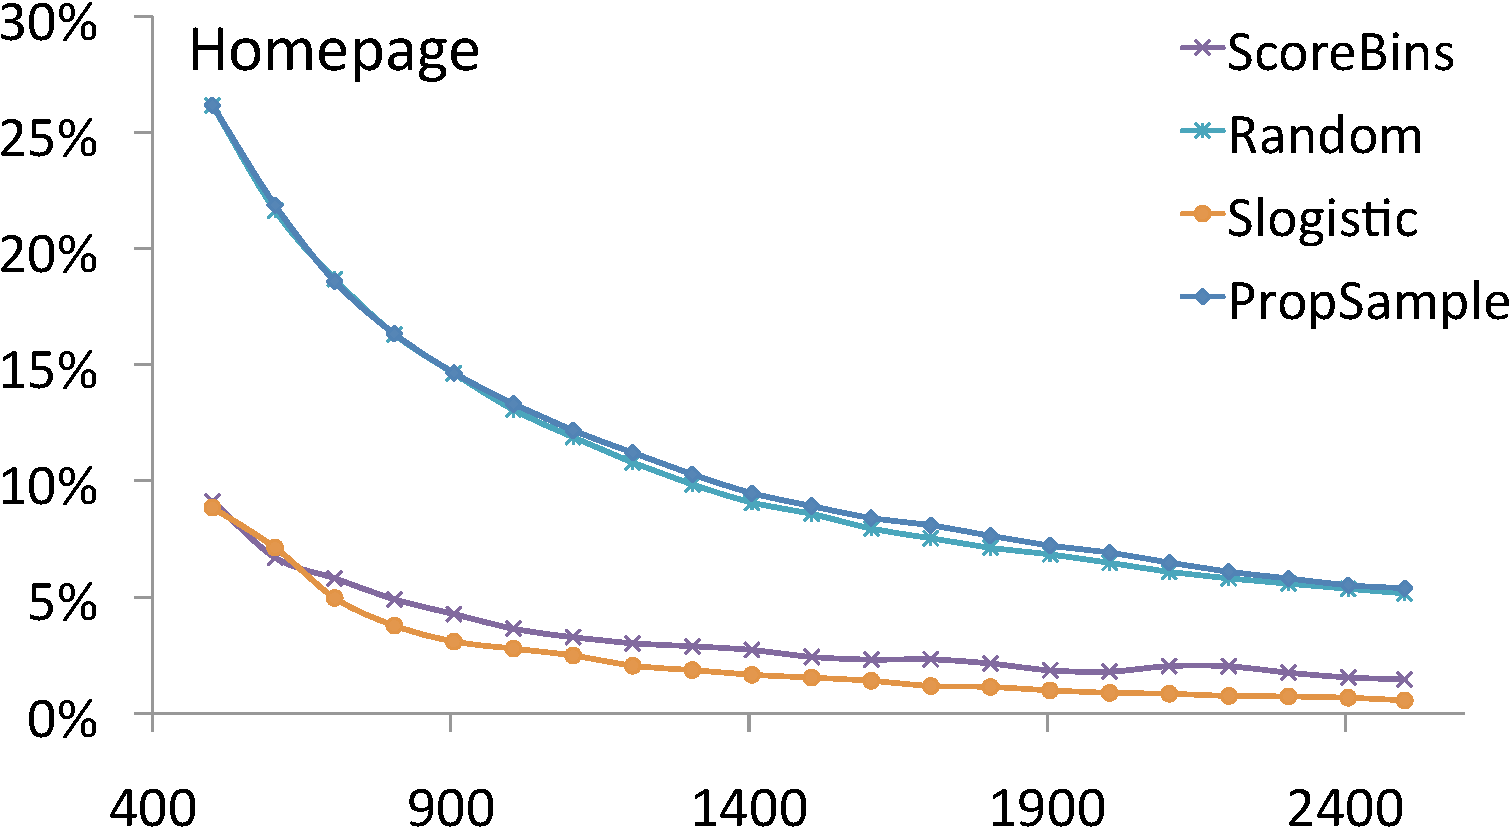
\includegraphics[width=0.35\hsize]{figs/e1ydatasetcrop}
%\end{center}
%\end{frame}
%
%% \subsection{Comparison of Stratification Methods}
%\begin{frame}
%\frametitle{Comaprison of Stratification Methods}
%\begin{center}
%\textsc{Error of different stratification methods against increasing training sizes \& for different no. of bits}
%\end{center}
%\begin{center}
%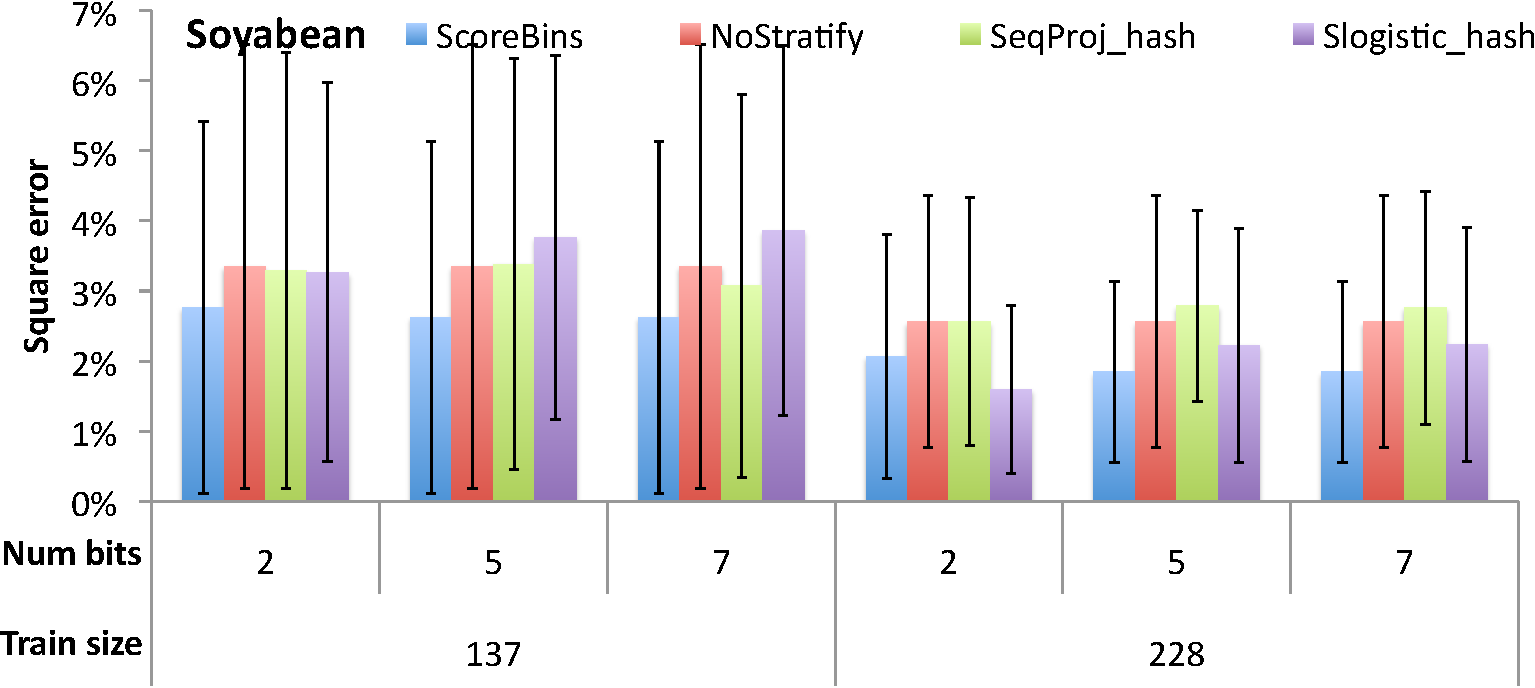
\includegraphics[width=0.34\hsize]{figs/e2wekacrop}
%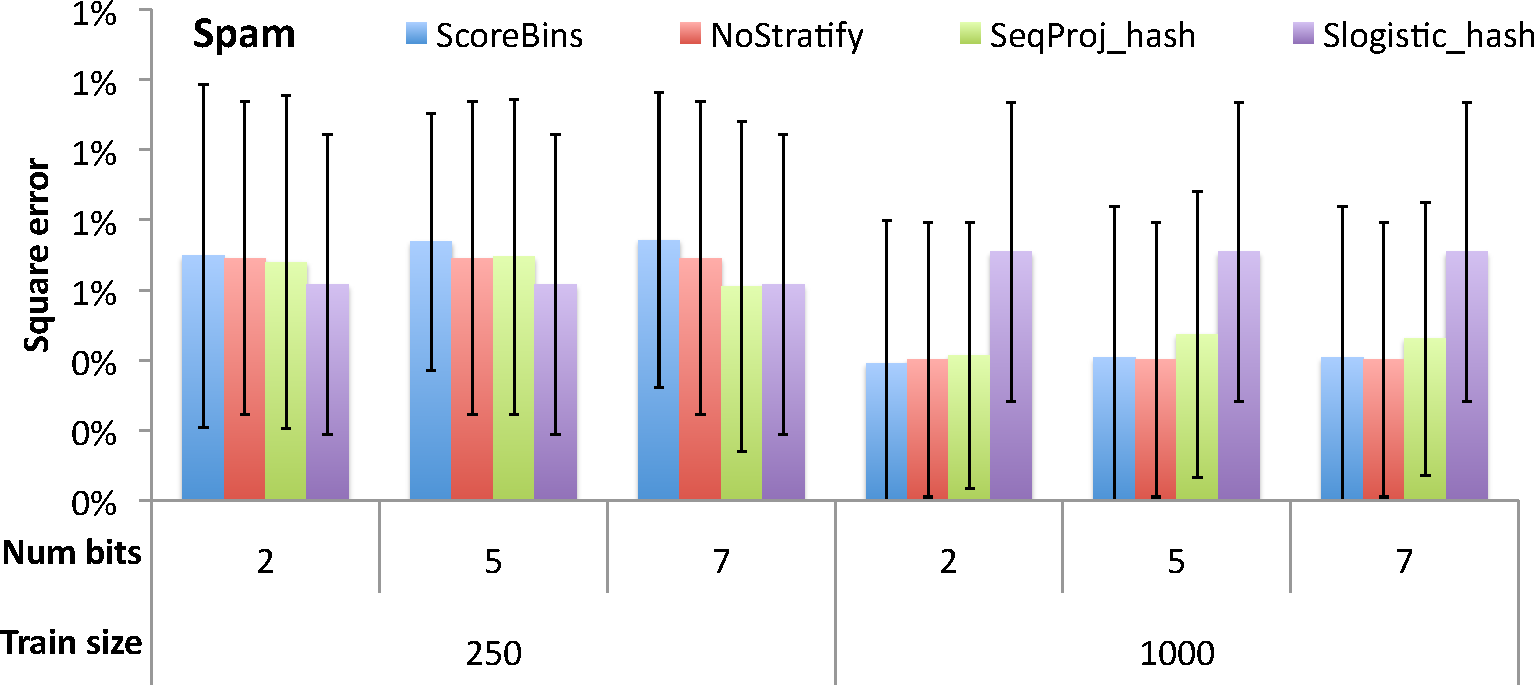
\includegraphics[width=0.34\hsize]{figs/e2webspamcrop}
%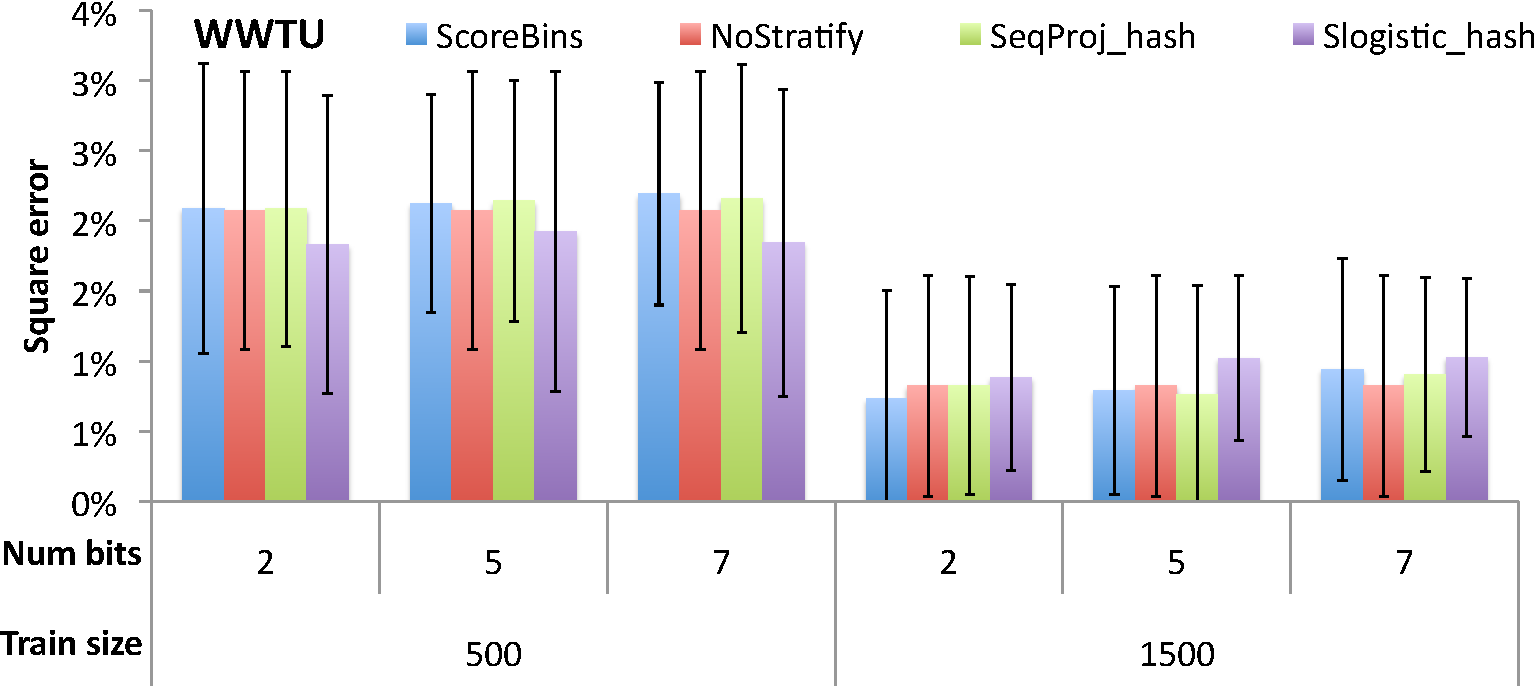
\includegraphics[width=0.34\hsize]{figs/e2wwtucrop}
%\end{center}
%\begin{center}
%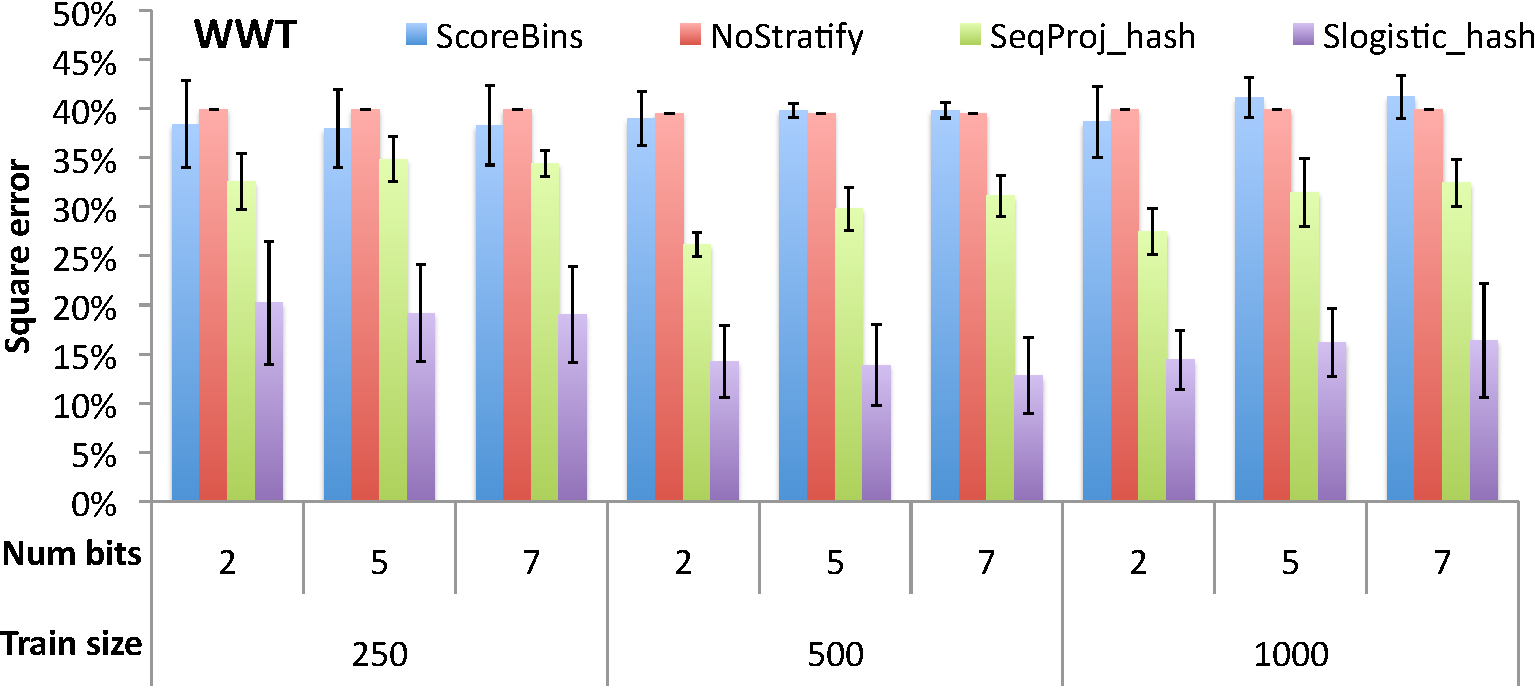
\includegraphics[width=0.42\hsize]{figs/e2wwtcrop}
%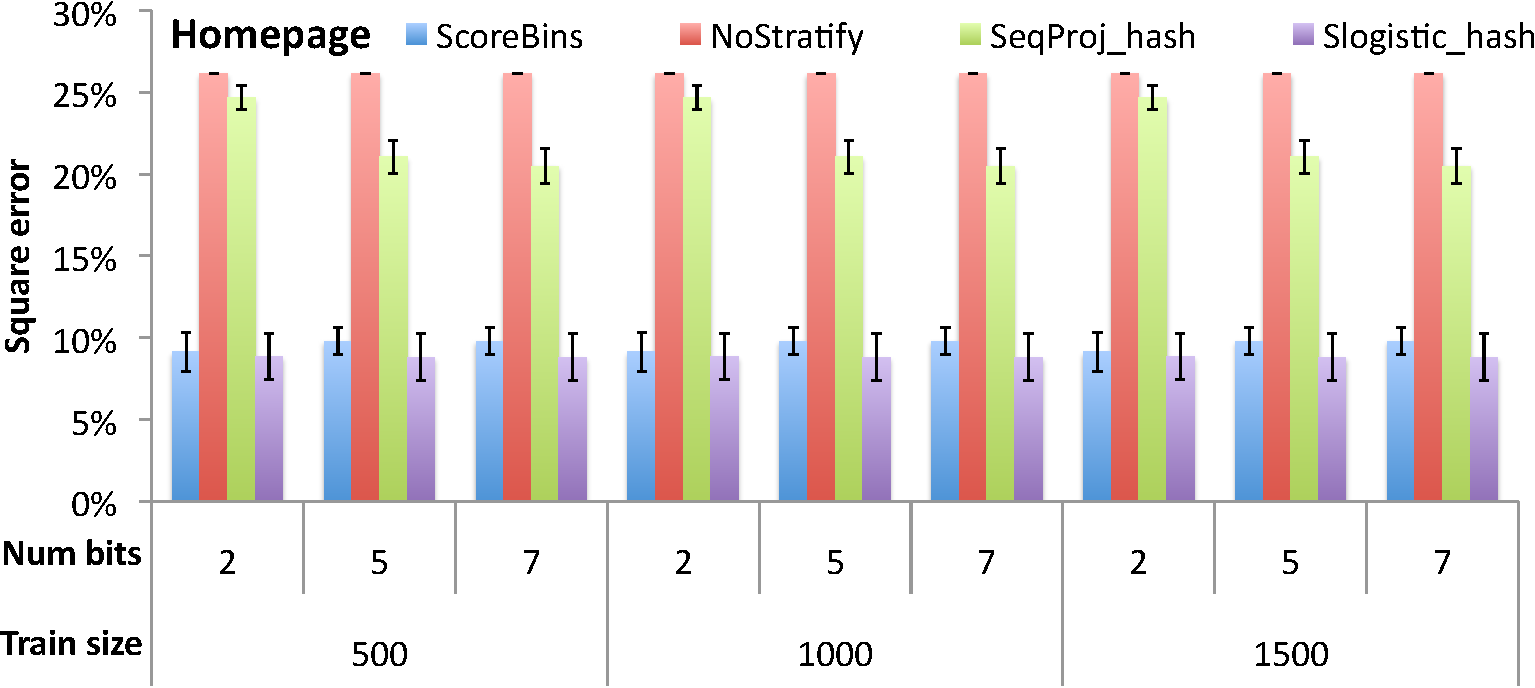
\includegraphics[width=0.42\hsize]{figs/e2ydatasetcrop}
%\end{center}
%\end{frame}
%
%% subsection{Efficiency of Indexed Data Access}
%\begin{frame}
%\frametitle{Efficiency of Indexed Data Access}
%\begin{center}
%\textsc{Comparing methods of sampling from indexed data for estimating bucket weights}
%\end{center}
%\begin{center}
%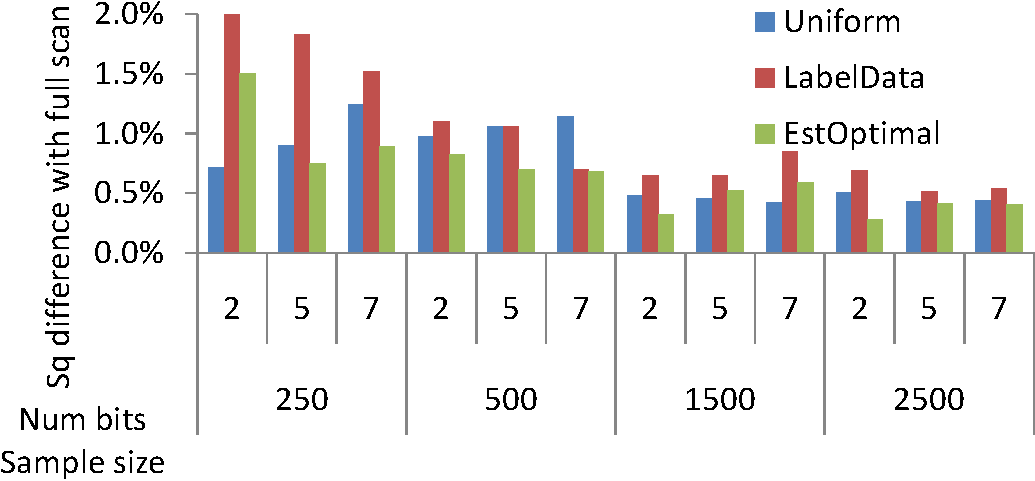
\includegraphics[width=0.45\hsize]{figs/allWts-crop}
%\end{center}
%\begin{center}
%\textsc{Error of different methods for selecting instances for labeling against increasing labeled data}
%\end{center}
%\begin{center}
%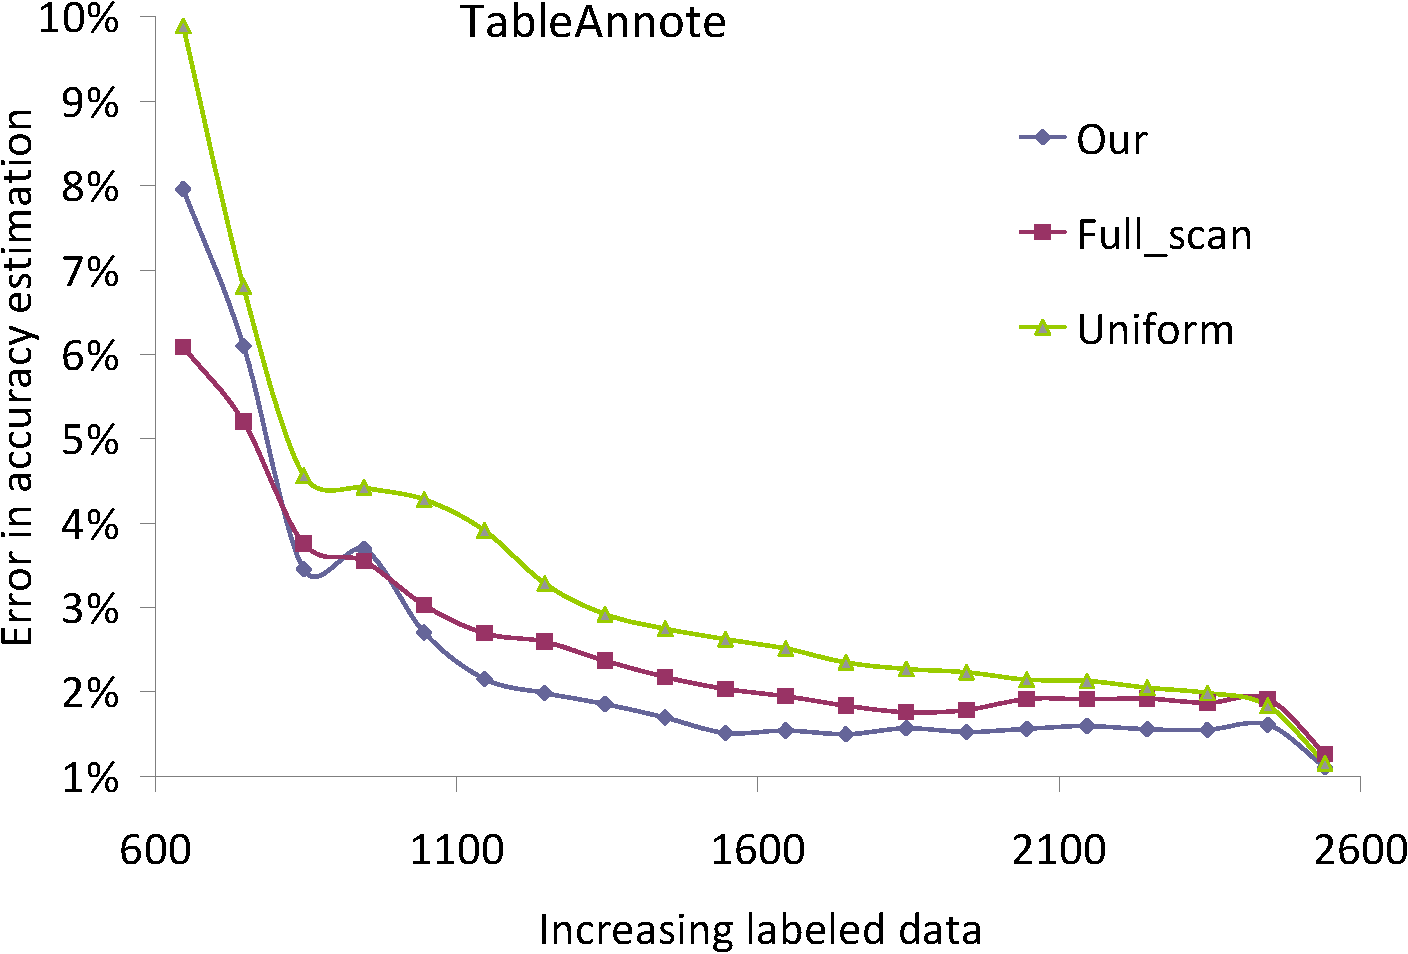
\includegraphics[width=0.30\hsize]{figs/selectB5-crop}
%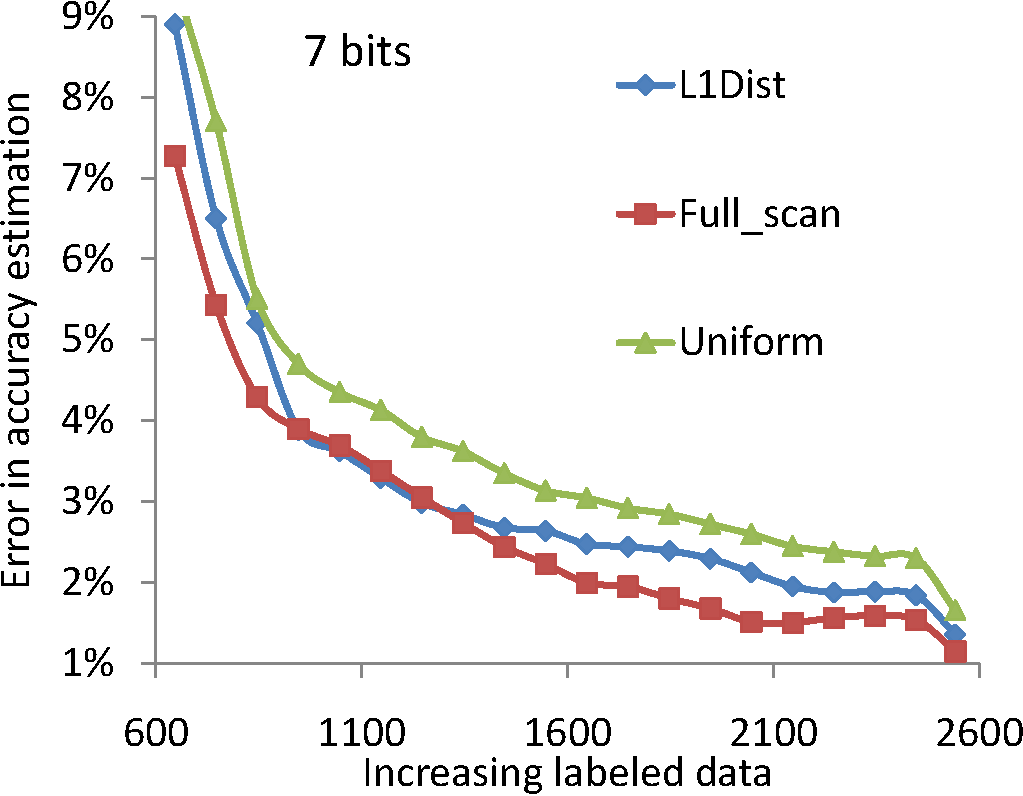
\includegraphics[width=0.30\hsize]{figs/selectB7-crop}
%\end{center}
%\end{frame}
%
%%%%%%%%%%%%%%%%%%%%%%%%%%%%%%%%%%%%%%%%%%%%%%%%%%%%%%%%%%%%%%%%%%%%%%%
%
%\section{Conclusions}
%\begin{frame}
%\frametitle{Conclusions}
%\begin{center}
%\begin{itemize}
%\item Proposed method of estimating the accuracy of a
%classifier on very large and diverse dataset  
%\item Method based on stratified sampling theory and makes following contributions beyond existing
%methods 
%\begin{itemize}
%\item Develop a stratification method based on $r$ bit
%signatures learned using a novel signed logistic algorithm
%\item Perform stratified sampling directly on indexed
%unlabeled data without requiring full data scan on every data
%re-stratification
%\end{itemize}
%\item Experiments on several real datasets show that our method provides
%more accurate estimates than existing methods, and that our strategies
%for accessing unlabeled data gives close to optimal performance while
%reading orders of magnitude fewer instances.
%\end{itemize}
%\end{center}
%\end{frame}